\minitoc
%\addcontentsline{toc}{section}{Dynamical systems} 

In this chapter we will learn about \textit{dynamical systems}, which can be very useful for modeling population dynamics. From one population to a system, we will review and explore models and methods to characterize and approximate population growth and decays.

\section{Modeling one population}
Suppose we want to track the evolution of one population. Choose one. Ready ? It can be whatever you want ! Let's denote $C(t)$ the number of individuals in that population at time $t$. We also assume $C(0)=2$. Why ? Because there is a need to have at least to individuals for growing (reproduction). The goal is to track the rate of change over time of the number of individuals. This implies that we're looking for a model of the form:
\[\displaystyle \frac{dC}{dt} = \mbox{growth model} = f(C,t), \quad C(0) =2 \]
\begin{itemize}
\item The above model represents an Initial Value Problem (IVP). Depending on the growth model $f$, one can make sure the mathematical model admits a unique solution. Picard's theorem, Lipschitz condition are for instance essential to assert existence and uniqueness (review concepts from math 24, math 125, math 131 or math 132 if needed).
\item All considered models in the chapter will be then first-order differential equations.
\item Depending on the sign of $f$, then we deduce if the population grows or decays. If $f >0$ then $\displaystyle \frac{dC}{dt} >0$ meaning $C$ grows, and vice versa.
\item It is important to keep in mind what the model is used for. For modeling a population growth, we can't have a negative number of individuals: $C(t) \geq 0$ at any time.
\end{itemize}

Let's start with the \textbf{exponential growth} model, also known as Malthus model:
\begin{equation}\label{:eq_exp_growth}
\displaystyle \frac{dC}{dt} = \alpha C ,\quad C(0) = 2 
\end{equation}
with $\alpha \neq 0$. If $\alpha>0$, it represents the growth rate, if $\alpha <0$ then it represents the decay rate. The above model is linear, separable, and the solution of \eqref{:eq_exp_growth} is given by (do you remember how to obtain this solution ?)
\[C(t) = 2 e^{\alpha t}\] 

It is commonly admitted that the exponential growth is not an adequate model: when growing, the population only grows, and very fast. But life can throw unexpected events, and death comes into play. A simple model that allows to take into account this \textbf{regulation} is the \textbf{logitstic growth} model, also known at Verhulst model:
\begin{equation}\label{:eq_logistic_growth}
\displaystyle \frac{dC}{dt} = \alpha C \left( 1 - \frac{C}{M} \right)  ,\quad C(0) = 2 
\end{equation}
with $\alpha >0$, and where $M >0$ represents the \textit{carrying capacity}. To understand what's the role of $M$, picture your flock of chickens ($C(t)$ for chicken right ?). Your backyard has limited space and you can't have hundreds of chickens there: there is not enough space, not enough food for all of them. Then $M$ represents the maximum number of chickens you can have.\\
In \eqref{:eq_logistic_growth} we have then $f(C,t) =f(C) =  \alpha C \left( 1 - \frac{C}{M} \right)$. Let's start by a qualitative analysis.
\begin{itemize}
\item Note that $f$ is a quadratic polynomial in $C$, $f(C) = 0 \Longleftrightarrow C = 0$ or $C = M$. Those two values represent the equilibrium points: $\displaystyle \frac{dC}{dt}  = 0$, so there is no rate of change (the number of chickens remains the same over time).
\item For $C <0$, then  $f(C) <0$ and the population decays. This case is not physically relevant.
\item For $C \in (0,M)$, then $f(C) >0$ and the population grows.
\item For $C >M$, then  $f(C) <0$ and the population decays. 
\item The equilibrium point $C = 0$ is unstable: close to it, the evolution of $C$ moves \textit{away} from it (grows or decays).
\item The equilibrium point $C = M$ is stable: close to it, the evolution of $C$ moves \textit{towards} it: increases until $C = M$, and decreases if over the carrying capacity.
\end{itemize}

\begin{Exercise}
The figure below represents $f$ for some $\alpha$ and $M $. Using the above remarks, identify (or provide an approximation of) $M$ and $\alpha$.\\
\begin{figure}[h!]
  \centering
  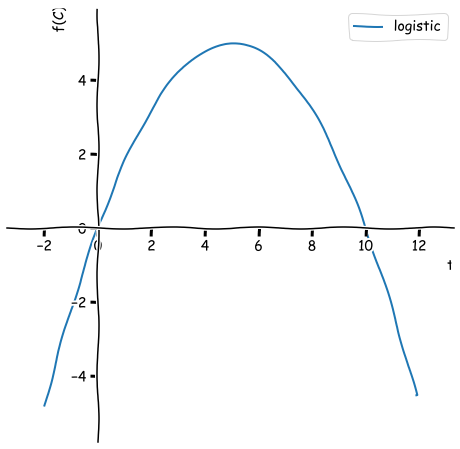
\includegraphics[width=0.4\linewidth]{img/logistic.png}
  \caption{Representation of the logistic growth rate for some $\alpha $ and $M$.}
  \label{fig:logistic}
 \end{figure}
 \dotfill

\dotfill

\dotfill

\dotfill

\dotfill

\dotfill

\dotfill

\dotfill

\dotfill

\dotfill
 \end{Exercise}
 
 Now let's solve \eqref{:eq_logistic_growth}. The equation is separable and we obtain:
 \[
\begin{aligned}
 \displaystyle & \frac{d C}{C(1 - \frac{C}{M})}  & = \alpha dt \\
 \displaystyle \Longleftrightarrow & \frac{M}{C(M -C)} dC & = \alpha dt \\
 \displaystyle \Longleftrightarrow & \left( \frac{1}{C } +  \frac{1}{M -C} \right) dC  & = \alpha dt \\
  \displaystyle \Longleftrightarrow & \frac{dC}{C } +  \frac{dC}{M -C}   & = \alpha dt \\
\end{aligned} 
 \]
 where we used the partial fraction decomposition. We can now easily integrate:
  \[
\begin{aligned}
  \displaystyle &  \int \frac{1}{C } dC + \int  \frac{1}{M -C} dC   & = \alpha \int dt \\
   \displaystyle \Longleftrightarrow & \ln |C| - \ln(|M-C|) & = \alpha t + c_0\\
      \displaystyle \Longleftrightarrow & \ln \frac{C}{|M-C|} & = \alpha t + c_0\\
\end{aligned} 
 \]
 with $c_0$ some integration constant. Note that, since we consider only $C \geq 0$ we can omit the absolute value in the numerator. Additionally, since $C = M$ is an equilibrium point (considered as maximum) let's assume we track $C \leq M$ so we can omit the absolute value in the denominator. Note as well $\ln$ or $\log$ do not matter here, we will consider the natural log for simplicity. Then we obtain
   \[
\begin{aligned}
      \displaystyle &  \frac{C}{M-C}  = e^{\alpha t + c_0} = c_1 e^{\alpha t }\\
       \displaystyle \Longleftrightarrow &  C (1 + c_1 e^{\alpha t }) = Mc_1 e^{\alpha t } \\
           \displaystyle \Longleftrightarrow &  C(t)  =  \frac{Mc_1 e^{\alpha t }}{(1 + c_1 e^{\alpha t })} \\   
\end{aligned} 
 \]
 with $c_1 = e^{c_0}$ a constant. Using the initial condition then we can find the constant $c_1$.
    \[
\begin{aligned}
      \displaystyle &  C(0) = 2 \\
       \displaystyle \Longleftrightarrow & \frac{Mc_1 e^{\alpha \times 0 }}{(1 + c_1 e^{\alpha \times 0 })} = 2  \\
           \displaystyle \Longleftrightarrow &  (M -2) c_1 = 2  \\   
              \displaystyle \Longleftrightarrow &c_1 = \frac{2}{M-2} \\   
\end{aligned} 
 \]
 Then the solution of \eqref{:eq_logistic_growth} is given by
 \[ C(t) = \displaystyle  \frac{2M}{M-2}\frac{e^{\alpha t }}{( 1+ \frac{2}{M-2} e^{\alpha t })}  \]
 Note that for a general initial condition $C(0)  = C_0$ then the solution of \eqref{:eq_logistic_growth} is given by
 \[ C(t) = \displaystyle  \frac{MC_0}{M-C_0}\frac{e^{\alpha t }}{( 1+ \frac{2C_0}{M-C_0} e^{\alpha t })}  \]
 \begin{Exercise}
 The figure below represents the evolution of $C(t)$ for various parameters. Comment the three graphs below: what do you conclude overall ?\\
 \begin{figure}[h!]
  \centering
  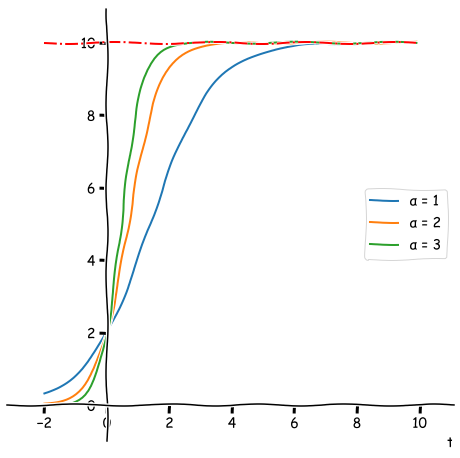
\includegraphics[width=0.3\linewidth]{img/logistic1.png}
    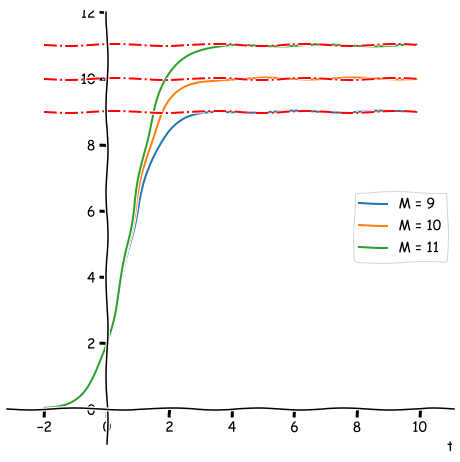
\includegraphics[width=0.3\linewidth]{img/logistic2.png}
      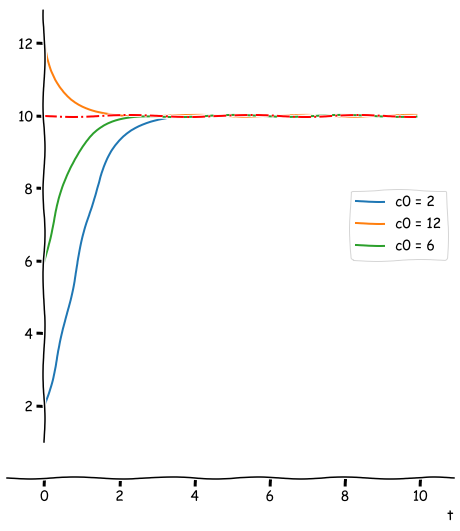
\includegraphics[width=0.3\linewidth]{img/logistic3.png}
  \caption{Evolution of the chickens population under logistic growth: (left) for various rates $\alpha$, (middle) for various carrying capacities $M$, (right) for various initial conditions $C_0$.}
  \label{fig:logistic}
 \end{figure}
  \dotfill

\dotfill

\dotfill

\dotfill

\dotfill

\dotfill

\dotfill

\dotfill

\dotfill

\dotfill
 \end{Exercise}
 
 There exists other models, such as the Gompertz model (see homework for more details). Now that we have one relevant model, let's investigate how to model multiple populations at the same time.
 
 \section{Modeling two populations: Competitive model}
 
 Consider now two populations, let's say $C(t)$ and $F(t)$. Both evolve over time and can be \textit{coupled}: each population affects the other. We will investigate both positive and negative effects. Let's start with the so-called \textbf{competitive model}:
 \begin{equation}\label{eq:competitive}
 \begin{aligned}
&\displaystyle \frac{dC}{dt} = \alpha_C C \left( 1 - \frac{C + \beta F}{M} \right)  ,\quad C(0) = C_0\\ 
&\displaystyle \frac{dF}{dt} = \alpha_F F \left( 1 - \frac{C + \beta F}{M} \right)  ,\quad F(0) = F_0
\end{aligned}
\end{equation}
with $\alpha_C, \alpha_F >0$ representing growth rates for each population, and $M >0$ representing now the total {carrying capacity} for both population. We assume both populations share the same resources and are bound to a specific ratio given by a new parameter, $\beta >0$. Note that when $\beta= 0$ then in \eqref{eq:competitive} boils down to
 \begin{equation}
 \begin{aligned}
&\displaystyle \frac{dC}{dt} = \alpha_C C \left( 1 - \frac{C }{M} \right)  ,\quad C(0) = C_0\\ 
&\displaystyle \frac{dF}{dt} = \alpha_F F \left( 1 - \frac{C }{M} \right)  ,\quad F(0) = F_0
\end{aligned}
\end{equation} 
The evolution of $C$ becomes the logistic growth, and $C$ affects the growth of $F$. Here \textbf{both populations grow !} Indeed even with $\beta = 0$, since we will work in the range $C \in (0, M)$ then $1 - \frac{C}{M} >0$, but can be small. In other words both populations grow but their growth rate is affected by the other population. $\beta$ allows to regulate this effect. There exist of course tons of different models, we consider here a simple one to introduce the idea of competition between species. \\ %Let's try now to solve this system.\\

Before jumping into solving an nonlinear ODE system (can you find why it is nonlinear ?), let's remark a couple of things. Note that:
\[
 \begin{aligned}
&\displaystyle \alpha_F F \frac{dC}{dt} = \alpha_C\alpha_F F C \left( 1 - \frac{C + \beta F}{M} \right)  ,\\
&\displaystyle  \alpha_C  C \frac{dF}{dt} =  \alpha_C\alpha_F F C \left( 1 - \frac{C + \beta F}{M} \right)  \\
\end{aligned}
\]
then both right-hand sides are equal, leading to
\[
 \begin{aligned}
 & \displaystyle \alpha_F F \frac{dC}{dt} -  \alpha_C  C \frac{dF}{dt} = 0\\
 \Longleftrightarrow \quad &  \displaystyle F \frac{dC}{dt} -  \frac{\alpha_C}{ \alpha_F}  C \frac{dF}{dt} = 0
\end{aligned} 
 \]
 Recall that quotient rule gives us
 \[ \left( \frac{f}{g^n} \right)' = \displaystyle \frac{f' g^n - n g^{n-1} g' f}{g^{2n}} = \frac{g^{n-1}}{g^{2n}} \left( f' g - n g'f \right)
 \]
then 
\[ \left( \frac{f}{g^n} \right)' = 0 \quad \Longleftrightarrow \quad  f' g - n g'f  = 0.\]
We obtain that
\[
 \begin{aligned}
  \displaystyle F C'-  \frac{\alpha_C}{ \alpha_F}  C F' = 0 \quad \Longleftrightarrow \quad \left( \frac{C}{F^{\frac{\alpha_C}{ \alpha_F} }} \right)' = 0 \quad  \Longrightarrow \quad  {C} = \gamma  F^{\frac{\alpha_C}{ \alpha_F} }
\end{aligned} 
 \]
with $\gamma$ a constant (assumed positive here for population tracking). It turns out $C$ and $F$ are proportional ! And it is now clear that both populations will grow with different rates:
\begin{itemize}
\item If $\frac{\alpha_C}{ \alpha_F}  > 1$, then $C$ grows much faster than $F$.
\item If $\frac{\alpha_C}{ \alpha_F}  < 1$, then $C$ grows much slower than $F$.
\item If $\frac{\alpha_C}{ \alpha_F}  = 1$, then $C$ grows at the same rate as $F$.
\end{itemize}
While we have two equations and two species, we can now reduce our system to a single ODE. Let's choose for example to replace $C$ and solve for $F$. We obtain:
\[\displaystyle  \frac{dF}{dt} =  \alpha_F F  \left( 1 - \frac{ \gamma  F^{\frac{\alpha_C}{ \alpha_F} } + \beta F}{M} \right) 
\]
Assume for now that $\frac{\alpha_C}{ \alpha_F}  = n >1$ an integer for simplicity. Then the above ODE admits at most $n+1$ equilibrium points. Indeed, the equilibrium points are found by solving
\[\displaystyle  \frac{dF}{dt} =   0  \quad \Longleftrightarrow \quad  F\left( - \frac{ \gamma}{M}  F^n + \frac{\beta}{M} F  +1\right)  = 0 \quad \Longleftrightarrow \quad  F \prod \limits_{i = 0}^{n-1} (F - F_i) = 0
\]
We can then rewrite the DE as 
\[
\displaystyle  \frac{dF}{dt} = \alpha_F F  \left( - \frac{ \gamma}{M}  F^n + \frac{\beta}{M} F  +1\right)  = - \frac{ \gamma  \alpha_F}{M} F\prod \limits_{i = 0}^{n-1} (F - F_i)  \]
which is a separable equation, and after tedious computations one can find the analytic solution. We do not pursue further here, it is a good practice to review how to solve differential equations though. The message to take here is the following: \textbf{do not rush into solving differential equations, analyze first. By analyzing we were able to reduce the system into a single differential equation}, and find that both population will grow with identified ratios. For more complicated system we will use numerical tools to solve it. We can for example use numerical schemes such as Euler's, Runge-Kutta (review math 130, math 131 or math 132). 
 \begin{Exercise}
 Repeat the procedure by choosing now to keep $C$ instead of $F$, and assume $\frac{\alpha_C}{ \alpha_F}  = \frac{1}{2}$. Find the equilibrium points and explain how you would proceed to find an analytic solution to the obtained DE.\\
  \dotfill

\dotfill

\dotfill

\dotfill

\dotfill

\dotfill

\dotfill

\dotfill

\dotfill

\dotfill
 \end{Exercise}

\section{Prey-predator model}

Our population of chickens and foxes ($F$ for fox, right ?) were increasing peacefully with the competitive model. But foxes eat chickens, so we need now to take into account the fact that there is a \textit{predator} and a \textit{prey}. The Lokta-Volterra model is a classic prey-predator model of the form:
 \begin{equation}\label{eq:prey-pred}
 \begin{aligned}
&\displaystyle \frac{dC}{dt} = \alpha C \left( 1 - \beta F\right)  ,\quad C(0) = C_0\\ 
&\displaystyle \frac{dF}{dt} = -  \delta F \left( 1 - \gamma C \right)  ,\quad F(0) = F_0,
\end{aligned}
\end{equation}
with $\alpha, \beta, \gamma, \delta >0$. $C$ represents the prey, and $F$ the predator. Let us make some remarks:
\begin{itemize}
\item $\alpha >0$ represents the growth rate of the population $C$
\item $- \delta < 0$ represents the \textit{decay} rate of the population $F$
\item both equations are coupled, the first equation has a coupling term $-\alpha \beta  CF <0$ (makes the population decay), the second equation has a coupling term $\delta \gamma CF >0$ (makes the population grow). In other words, the predator population seems to grow in presence of preys, and the prey population decays in presence of predators. The model is then consistent with what we plan to model.
\item $\beta$ and $\gamma$ play a role of turning points. Qualitatively, if we look at the first equation, when $F < \frac{1}{\beta}$ then $  \alpha C \left( 1 - \beta F\right) >0$ meaning the population $C$ grows. There are not enough foxes to eat all chickens, the population can grow. If $F > \frac{1}{\beta}$ then $  \alpha C \left( 1 - \beta F\right) <0$ meaning the population $C$ decays. There are enough foxes to eat chickens, the population decays. Similarly, when $C < \frac{1}{\gamma}$ then $  -  \delta F \left( 1 - \gamma C \right) < 0$ meaning the population $F$ decays. There are not enough chickens to feed all foxes, the population decays. If $C > \frac{1}{\gamma}$ then $  -  \delta F \left( 1 - \gamma C \right) >0$ meaning the population $F$ grows. There are enough chickens to feed the foxes, the population grows.
\end{itemize}
We can now study the system following standard procedure for systems of first-order ODEs. This includes
\begin{enumerate}
\item Find equilibrium points
\item Linearize the system at each equilibrium point
\item Study the stability of each equilibrium point via the linearized system
\item Gather all information into the phase portrait
\end{enumerate}
We will apply those 4 items for each system. \textbf{You will be required to follow the same procedure if you consider a model problem based on a system of first-order differential equations.}\\

\begin{remark}
The above procedure can be as well applied to the competitive model. It is a good exercise to try afterwards.
\end{remark}

\subsection{Equilibrium points} One can see that there are two equilibrium points (do you remember how to find them ?)
\[ \displaystyle \frac{dC}{dt} =\displaystyle \frac{dF}{dt}  =  0  \quad \Longleftrightarrow \quad (C,F) = (0,0), \quad  (C,F) = (\frac{1}{\gamma},\frac{1}{\beta}) \]
Recall that an equilibrium point is such that \textbf{both equations are equal to $0$ simultaneously}. Make sure to check that before moving to the next step ! 
 \begin{Exercise}
Find the equilibrium points of the system 
\[ \begin{aligned}
&\displaystyle \frac{dx}{dt} = x \left( 1 -x - 2y \right)  
&\displaystyle \frac{dy}{dt} = y \left( 1 -2x -2 y \right) 
\end{aligned}
\]
  \dotfill

\dotfill

\dotfill

\dotfill

\dotfill

\dotfill

\dotfill

\dotfill

\dotfill

\dotfill
 \end{Exercise}
 
\subsection{Linearize the system} Linearizing the system stands for considering a linear approximation of the differential equation. From vector calculus you learned that the linear approximation of a 2-variable function at a point is given by its tangent plane. That means that 
\[ f(x,y) \approx  f(x_0,y_0) + \frac{\partial f}{\partial x}(x_0,y_0) [x- x_0] + \frac{\partial f}{\partial y}(x_0,y_0) [y- y_0]\]
Then for a system of the form
\[
\begin{aligned}
& \displaystyle \frac{d x}{dt} = f(x,y)\\
& \displaystyle \frac{d y}{dt} = g(x,y)\\
\end{aligned}
\]
The linear approximation at a point $(x,y) = (x_0,y_0)$ is given by
\[
\begin{aligned}
& \displaystyle \frac{d x}{dt}  \approx  f(x_0,y_0) + \frac{\partial f}{\partial x}(x_0,y_0) [x- x_0] + \frac{\partial f}{\partial y}(x_0,y_0) [y- y_0]\\
& \displaystyle \frac{d y}{dt}  \approx  g(x_0,y_0) + \frac{\partial g}{\partial x}(x_0,y_0) [x- x_0] + \frac{\partial g}{\partial y}(x_0,y_0) [y- y_0]\\
\end{aligned}
\]
Suppose that the point $(x_0,y_0)$ is an equilibrium point. That means that $\frac{d x_0}{dt}  = f(x_0,y_0) =  0 = \frac{d y_0}{dt}  = g(x_0,y_0)  $, and we can write the above system as 
\[ 
\displaystyle \frac{d }{dt} \begin{pmatrix}
x - x_0 \\y - y_0
\end{pmatrix} = \begin{bmatrix}
\displaystyle\frac{\partial f}{\partial x}(x_0,y_0) &\displaystyle  \frac{\partial f}{\partial y}(x_0,y_0)\\
\displaystyle\frac{\partial g}{\partial x}(x_0,y_0) &\displaystyle \frac{\partial g}{\partial y}(x_0,y_0)
\end{bmatrix} \begin{pmatrix}
x -x_0\\y- y_0
\end{pmatrix} \quad \Longleftrightarrow \quad  X' = A X
\]
with $A$ the Jacobian matrix of the linearized system. We may now simply study the linear system $ X' = A X$ to investigate the stability of each equilibrium point. Note that each equilibrium point provides a system, \textbf{you will repeat the procedure as many times as there are equilibrium points}. For each linearized system, $0$ now corresponds to the new equilibrium ($X = 0 \Longleftrightarrow (x,y) = (x_0,y_0)$).\\

\begin{remark}
The Jacobian matrix is not limited to systems 2D. Given a $N \times N$  system of first-order differential equations
\[
\begin{aligned}
 \displaystyle \frac{d y_1}{dt}  & = f_n(y_1, \dots, y_n, t)\\
\vdots & \qquad \vdots\\
 \displaystyle \frac{d y_n}{dt}  & = f_n(y_1, \dots, y_n, t)\\
\end{aligned}
\]
then the Jacobian matrix at a point $Y_0 = (y_{1,0}, \dots, y_{n,0})$ is given by
\[A_{Y_0} =  \begin{bmatrix}
\displaystyle\frac{\partial f_1}{\partial y_1}(Y_0)  & \dots & \dots & \dots  & \displaystyle\frac{\partial f_1}{\partial y_n}(Y_0)   \\
 \vdots & \ddots  & \ddots  & \ddots & \vdots  \\
 \vdots  &\displaystyle\frac{\partial f_i}{\partial y_{i-1}}(Y_0)  &\displaystyle\frac{\partial f_i}{\partial y_i}(Y_0)  & \displaystyle\frac{\partial f_i}{\partial y_{i+1}}(Y_0)   & \vdots\\
  \vdots  & \ddots  &\ddots & \ddots  & \vdots \\
\displaystyle\frac{\partial f_n}{\partial y_1}(Y_0)     & \dots & \dots  & \dots &  \displaystyle\frac{\partial f_n}{\partial y_n}(Y_0)  \\
\end{bmatrix} .
\]
\end{remark}


Back to our prey-predator model we have
\[
 \begin{aligned}
&\displaystyle \frac{dC}{dt} = \alpha C \left( 1 - \beta F\right)  = f(C,F)\\ 
&\displaystyle \frac{dF}{dt} = -  \delta F \left( 1 - \gamma C \right)  = g(C,F)
\end{aligned}
\]
Then our jacobian matrix becomes at an equilibrium point $(C_{eq}, F_{eq})$
\[ A_{(C_{eq}, F_{eq})} =   \begin{bmatrix}\displaystyle
\frac{\partial f}{\partial C}(C_{eq}, F_{eq})&  \displaystyle\frac{\partial f}{\partial F}(C_{eq}, F_{eq})\\
\displaystyle \frac{\partial g}{\partial C}(C_{eq}, F_{eq}) &  \displaystyle\frac{\partial g}{\partial F}(C_{eq}, F_{eq})
\end{bmatrix}   =  \begin{bmatrix}
\alpha (1 - \beta F_{eq})& - \beta \alpha C_{eq} \\
\delta \gamma F_{eq})&-\delta (1 - \gamma C_{eq})\\
\end{bmatrix}\]

We have identified two equilibrium points $(C_{eq},F_{eq}) = (0,0)$, $(C_{eq},F_{eq}) = (\frac{1}{\gamma},\frac{1}{\beta})$. We obtain two linear systems:
\[ 
\displaystyle \frac{d }{dt} \begin{pmatrix}
C \\F 
\end{pmatrix} = A_{(0,0)} \begin{pmatrix}
C\\F
\end{pmatrix} = \displaystyle  \begin{bmatrix}
\alpha & 0 \\
0&-\delta \\
\end{bmatrix} \begin{pmatrix}
C\\F
\end{pmatrix},
\]
\[ \displaystyle \frac{d }{dt} \begin{pmatrix}
C - \frac{1}{\gamma} \\F - \frac{1}{\beta} 
\end{pmatrix} = A_{(\frac{1}{\gamma},\frac{1}{\beta})}  \begin{pmatrix}
C - \frac{1}{\gamma} \\F - \frac{1}{\beta} 
\end{pmatrix} =   \begin{bmatrix}
0& \displaystyle- \frac{\beta \alpha }{\gamma} \\
 \displaystyle\frac{\delta \gamma}{\beta}&0\\
\end{bmatrix}  \begin{pmatrix}
C - \frac{1}{\gamma} \\F - \frac{1}{\beta} 
\end{pmatrix} .\]

 \begin{Exercise}
Write the associated linear system to each equilibrium point found previously for the system
\[ \begin{aligned}
&\displaystyle \frac{dx}{dt} = x \left( 1 -x - 2y \right)  
&\displaystyle \frac{dy}{dt} = y \left( 1 -2x -2 y \right) 
\end{aligned}
\]
  \dotfill

\dotfill

\dotfill

\dotfill

\dotfill

\dotfill

\dotfill

\dotfill

\dotfill

\dotfill
 \end{Exercise}

\subsection{Stability of the equilibria} From your differential equation course (math 24 or math 125) you learned that stability of equilibrium points of autonomous linear systems are related to eigenvalues of the matrix system. Given a system 
\[X' = A X\]
then we will investigate the sign of the eigenvalues of the matrix $A$ to determine stability of the system. This comes from the following observation. Given $A \in \mathbb{R}^{N \times N}$ a squared matrix, if $A$ is diagonalizable (in $\mathbb{R}$ or $\mathbb{C}$) then $A$ admits $N$ eigenvalues $\lambda_i$, $i = 1 , \dots, N$ (they can be repeated but the dimension of eigenspace matches the number of repetition here) and we write 
\[A = P^{-1} \begin{bmatrix}
\lambda_1 & 0 & \dots & \dots  & 0  \\
0 & \ddots  & \ddots  & \ddots & \vdots  \\
 \vdots  & \ddots &\lambda_i & \ddots  & 0\\
  \vdots  & \ddots  &\ddots & \ddots  & \vdots \\
0   & \dots & \dots  & 0 &  \lambda_N \\
\end{bmatrix} P
\]
with $P\in \mathbb{R}^{N \times N}$ an orthonormal matrix. Plugging this representation into our linear system gives us:
\[ X' = A X \quad \Longleftrightarrow \quad  (PX)' =  \begin{bmatrix}
\lambda_1 & 0 & \dots & \dots  & 0  \\
0 & \ddots  & \ddots  & \ddots & \vdots  \\
 \vdots  & \ddots &\lambda_i & \ddots  & 0\\
  \vdots  & \ddots  &\ddots & \ddots  & \vdots \\
0   & \dots & \dots  & 0 &  \lambda_N \\
\end{bmatrix}  PX\]
Denoting $Y = PX \in \mathbb{R}^N = (y_1, \dots, y_N)$ we obtained the linear system:
\[
\begin{aligned}
 y_1' &= \lambda_1 y_1 \\
 \vdots & \quad \vdots  \\
 y_N' &= \lambda_N y_N \\
\end{aligned}
\quad  \Longrightarrow  \quad 
\begin{aligned}
  y_1(t)  &= y_1(0) e^{\lambda_1 t}=  y_1(0) e^{\Re(\lambda_1) t} (\cos (\Im(\lambda_1) t) + i \sin (\Im(\lambda_1) t) )\\
 \vdots & \qquad \qquad   \vdots  \\
 y_N(t) &= y_N(0) e^{\lambda_N t}=  y_N(0) e^{\Re(\lambda_N) t} (\cos (\Im(\lambda_N) t) + i \sin (\Im(\lambda_N) t) )\\
\end{aligned}
\]
and it is now straightforward to investigate the stability of the equilibrium point $0$.
\begin{itemize}
\item If $\Re (\lambda_i) <0$ for all $i = 1, \dots, N$ then the equilibrium is \textit{asymptotically stable}. All components are exponentially decreasing towards $0$ as $t \to \infty$.
\item If there exists $j \in \llbracket 1, N \rrbracket$ such that $\Re (\lambda_j) >0$ then the equilibrium is \textit{unstable}. The $j$th component is exponentially increasing to $\infty$ as $t \to \infty$.
\item If $\Re (\lambda_i) = 0$ for all $i = 1, \dots, N$ then the equilibrium is \textit{marginally stable}. All components remain bounded as $t \to \infty$ (rotation).
\end{itemize}

\begin{remark}
The above results regarding stability are valid even if the matrix $A$ is non diagonalizable (the dimension of the eigenspace doesn't match the eigenvalues' multiplicity). In that case the matrix always admits a Jordan form:
\[A = P^{-1} \begin{bmatrix}
J_1 & 0 & \dots & \dots  & 0  \\
0 & \ddots  & \ddots  & \ddots & \vdots  \\
 \vdots  & \ddots &J_i & \ddots  & 0\\
  \vdots  & \ddots  &\ddots & \ddots  & \vdots \\
0   & \dots & \dots  & 0 & J_M \\
\end{bmatrix} P,
\]
where $J_i$, $i = 1, \dots, P$ are block matrices of the form $J_i = \lambda_i I + N_i$ ($\lambda_i$ on the diagonal and an upper triangular Nilpotent matrix). The obtained solution of the system now contains terms of the form $ e^{\lambda_i t}$, $t e^{\lambda_i t}$, $t^2 e^{\lambda_i t}$, all driven by the same exponential.
\end{remark}

Back to our prey-predator model we have:
\[A_{(0,0)}  = \displaystyle  \begin{bmatrix}
\alpha & 0 \\
0&-\delta \\
\end{bmatrix} \]
is already diagonal and admits $\lambda_1 = \alpha >0$, $\lambda_2 = -\delta <0$ as eigenvalues. Because $\lambda_1 >0$, $(0,0)$ is an unstable equilibrium point. \\
For 
\[ A_{(\frac{1}{\gamma},\frac{1}{\beta})}=   \begin{bmatrix}
0& \displaystyle- \frac{\beta \alpha }{\gamma} \\
 \displaystyle\frac{\delta \gamma}{\beta}&0\\
\end{bmatrix} 
\]
we find 
\[ 
det (A_{(\frac{1}{\gamma},\frac{1}{\beta})} - \lambda I) = 0  \quad \Longleftrightarrow \quad \lambda^2 + \delta \alpha = 0
\]
which provides $\lambda = \pm i \sqrt{\delta \alpha}$. Both roots are pure imaginary, $\Re(\lambda) = 0$, the equilibrium point $(\frac{1}{\gamma},\frac{1}{\beta})$ is then marginally stable.

 \begin{Exercise}
For the system
\[ \begin{aligned}
&\displaystyle \frac{dx}{dt} = x \left( 1 -x - 2y \right)  
&\displaystyle \frac{dy}{dt} = y \left( 1 -2x -2 y \right) 
\end{aligned}
\]
determine the stability of the each equilibrium point found previously.\\
  \dotfill

\dotfill

\dotfill

\dotfill

\dotfill

\dotfill

\dotfill

\dotfill

\dotfill

\dotfill
 \end{Exercise}

\subsection{Phase portrait}
Once we have identified stability of the equilibrium we can then have an idea of the trajectories in the vicinity of each equilibrium point: plotting those trajectories represents the phase portrait. While it may be difficult to visualize a phase portrait in $N$ dimensions (for a $N \times N$ system), it is much easier in the case of a $2 \times 2$ system. We provide in Figure \ref{fig:root1} a summary of all possible phase portraits one can expect around an equilibrium point for a system 2D.\\

Back to our prey-predator model we found
\begin{itemize}
\item 2 distinct real roots around $(0,0)$ with one positive.
\item 2 pure imaginary roots around $(\frac{1}{\gamma},\frac{1}{\beta})$.
\end{itemize}
We obtain then the following portrait (see Figure \ref{fig:phase}): both populations oscillate around the equilibrium point $(\frac{1}{\gamma},\frac{1}{\beta})$, without chickens the population of foxes decays, without foxes the population of chickens thrives. Let us note that bounded trajectories don't have to be ellipses or circles. You may have obtained such trajectories when solving the system for the unknown $Y = PX$, but not anymore when back to our unknowns $X = (C,F)$. Note that both plots in Figure \ref{fig:phase} represent the same information (one trajectory) but with a different point of view. Using both representations is important, especially for larger systems (where a $N$-dimensional phase portrait might be difficult to plot).
 \begin{figure}[h!]
  \centering
  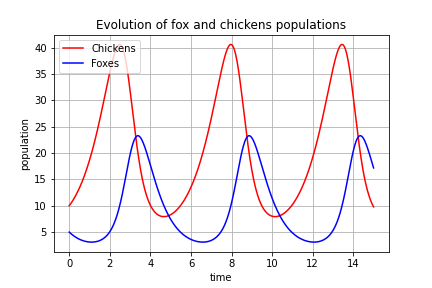
\includegraphics[width=0.49\linewidth]{img/chickens_and_foxes_1.png}
    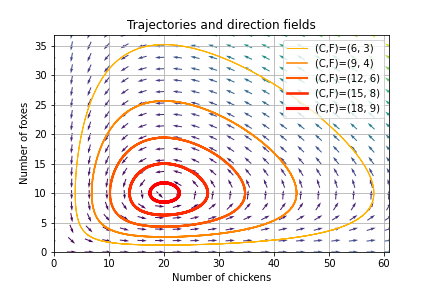
\includegraphics[width=0.49\linewidth]{img/chickens_and_foxes_2.png}
  \caption{(Left) Evolution over time of $C(t)$, $F(t)$ for some given $\alpha, \beta, \gamma, \delta$ and some initial condition. (Right) Phase portrait $(C(t), F(t))$ with some trajectories and direction field for some given $\alpha, \beta, \gamma, \delta$.}
  \label{fig:phase}
 \end{figure}
 
  \begin{Exercise}
  Determine the values of $\beta, \gamma$ used to obtain the phase portrait in Firgure \ref{fig:phase}.
  \dotfill

\dotfill

\dotfill

\dotfill

\dotfill

\dotfill

\dotfill

\dotfill

\dotfill

\dotfill
 \end{Exercise}
 \begin{figure}[H]
  \centering
  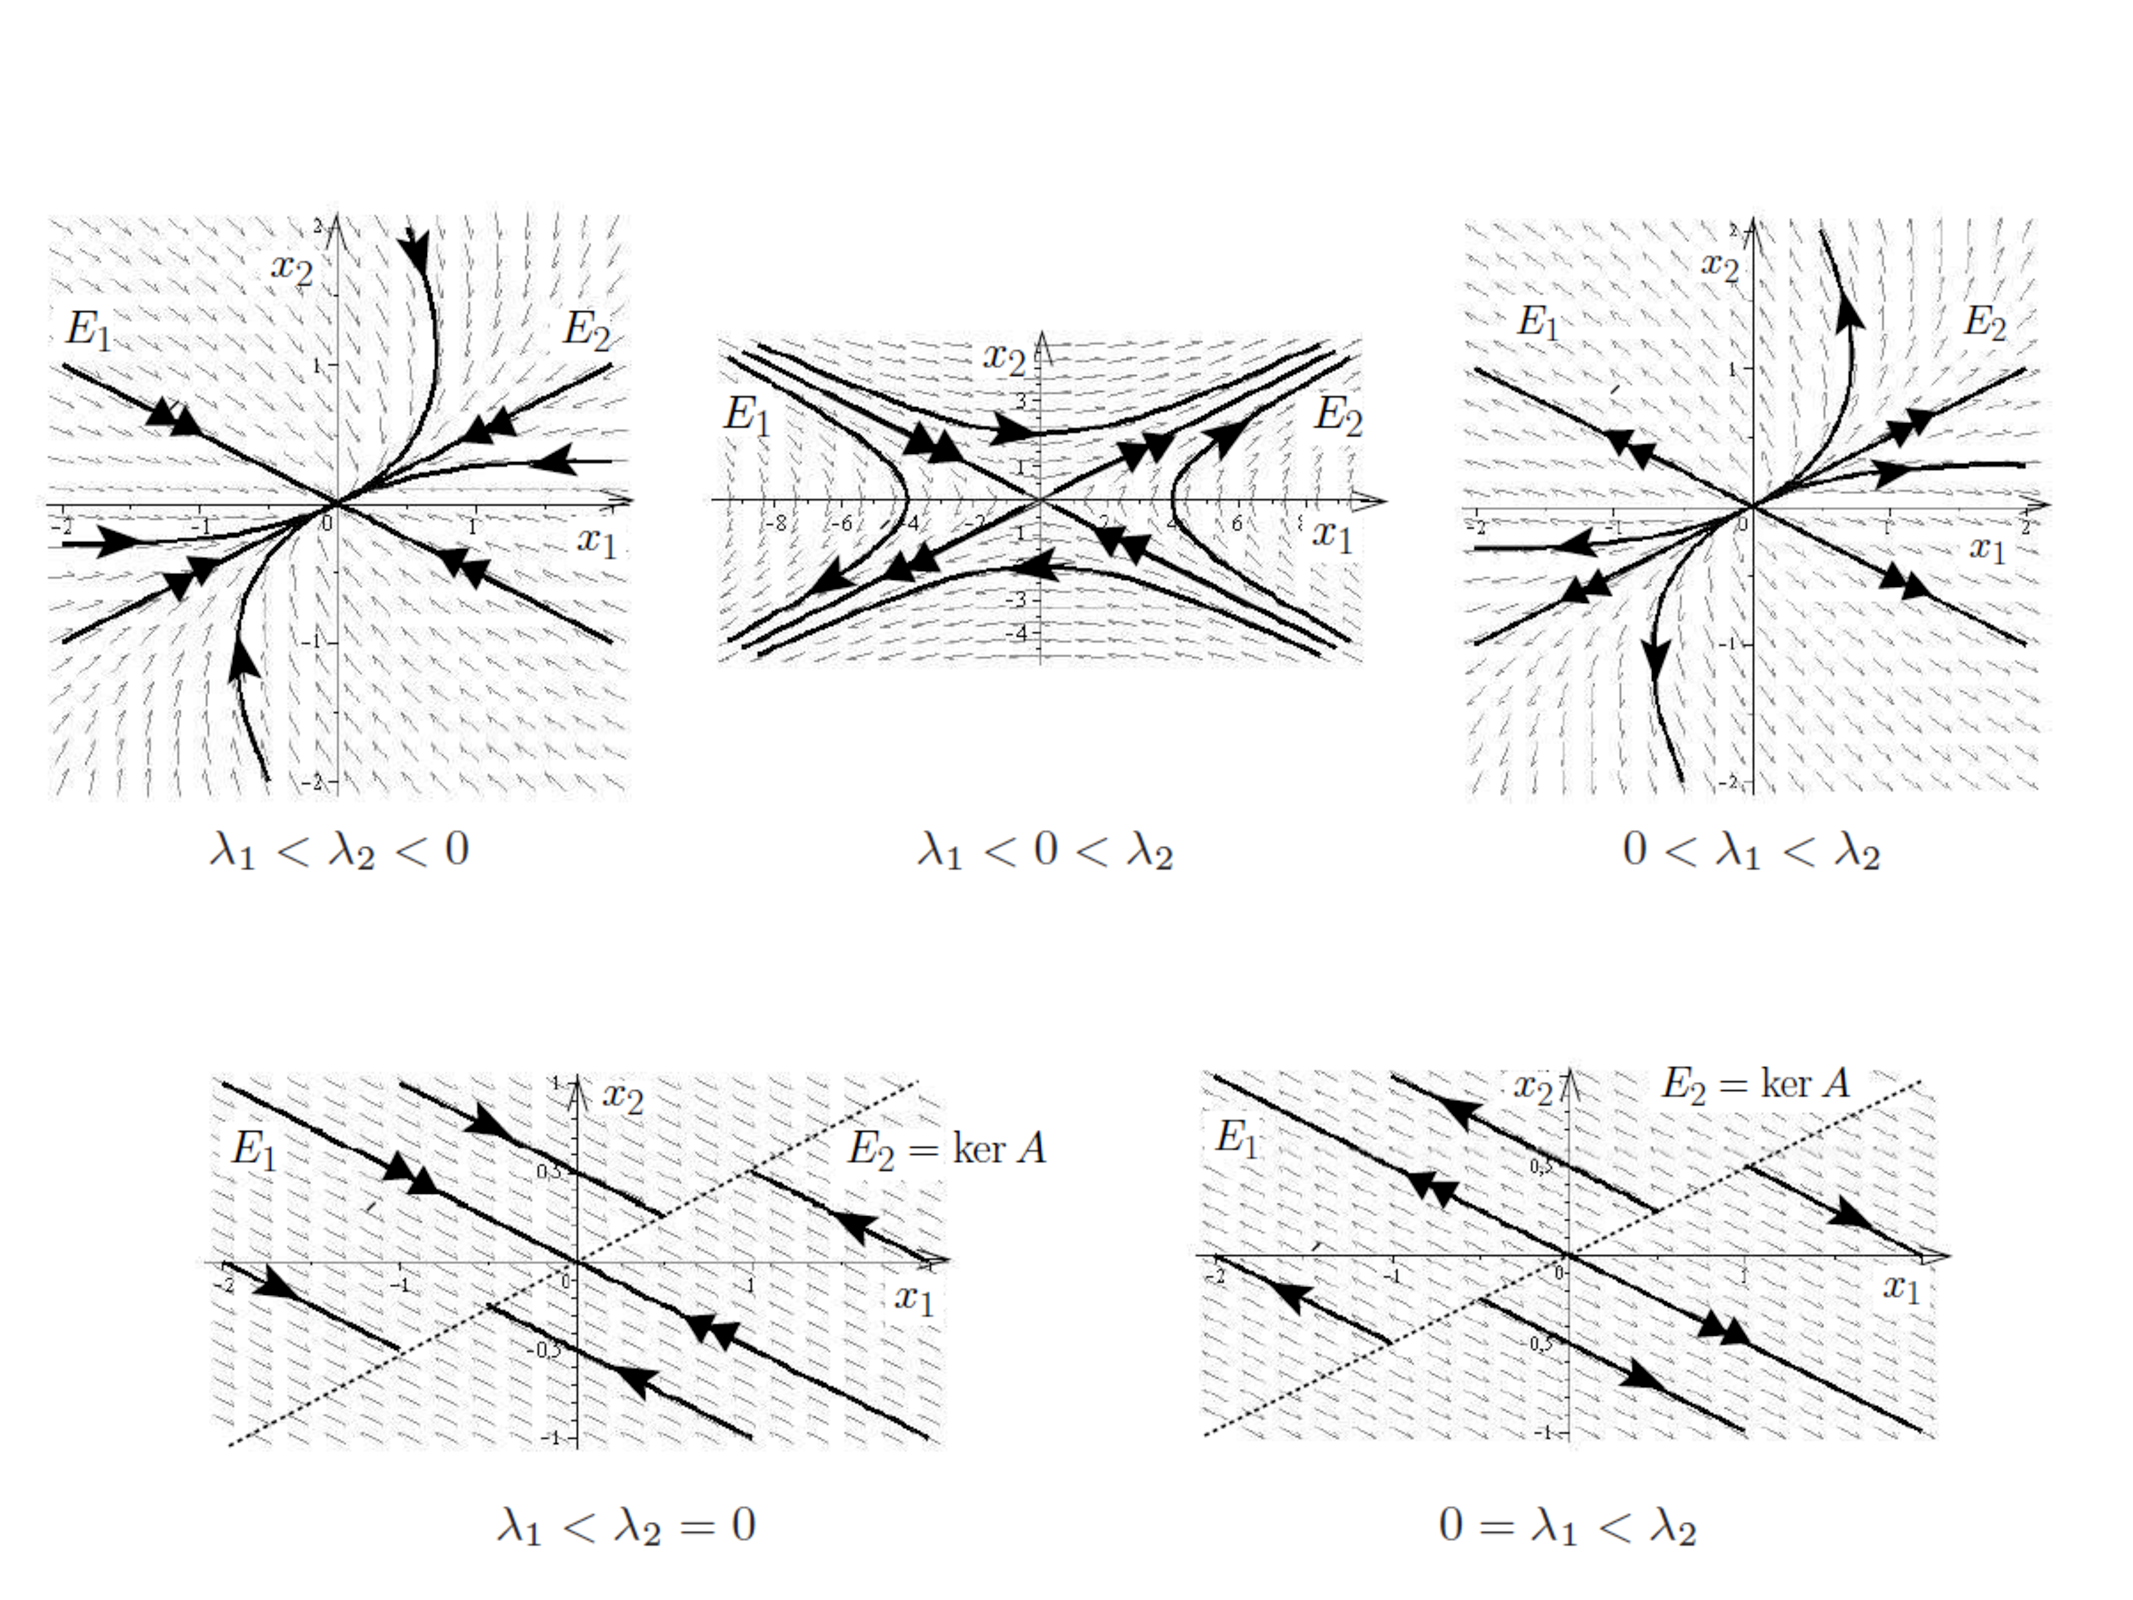
\includegraphics[width=0.7\linewidth]{img/root1.pdf}\\
    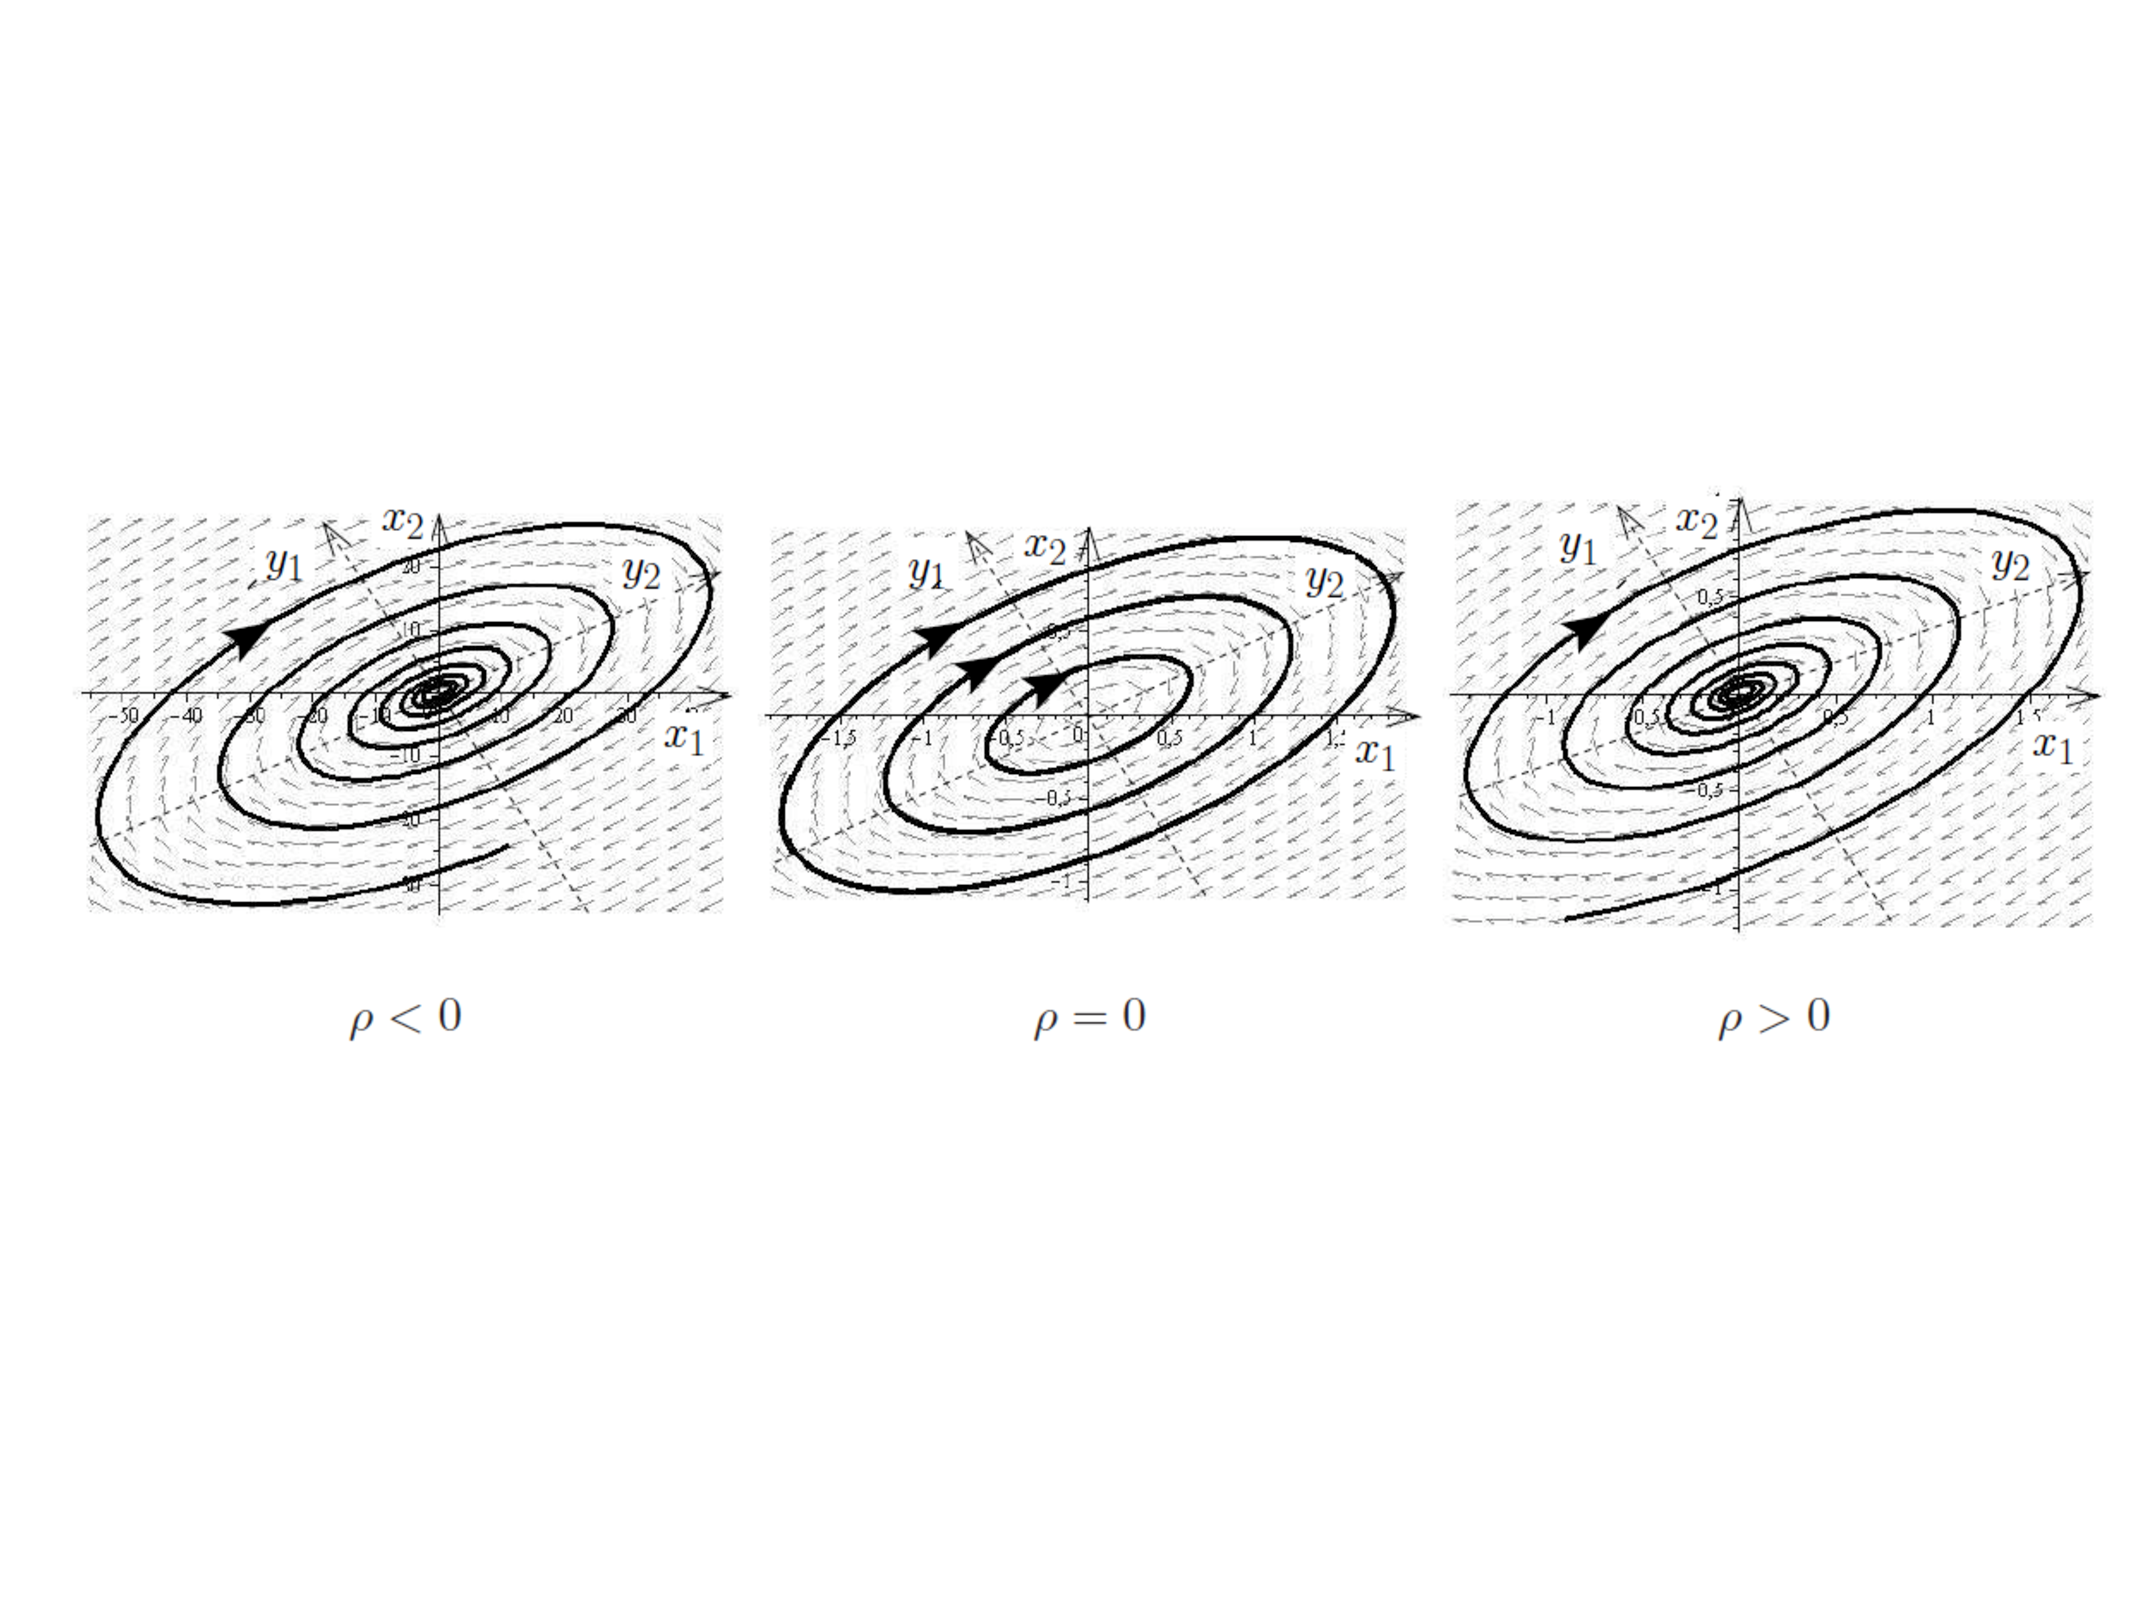
\includegraphics[width=0.7\linewidth]{img/root2.pdf}\\
      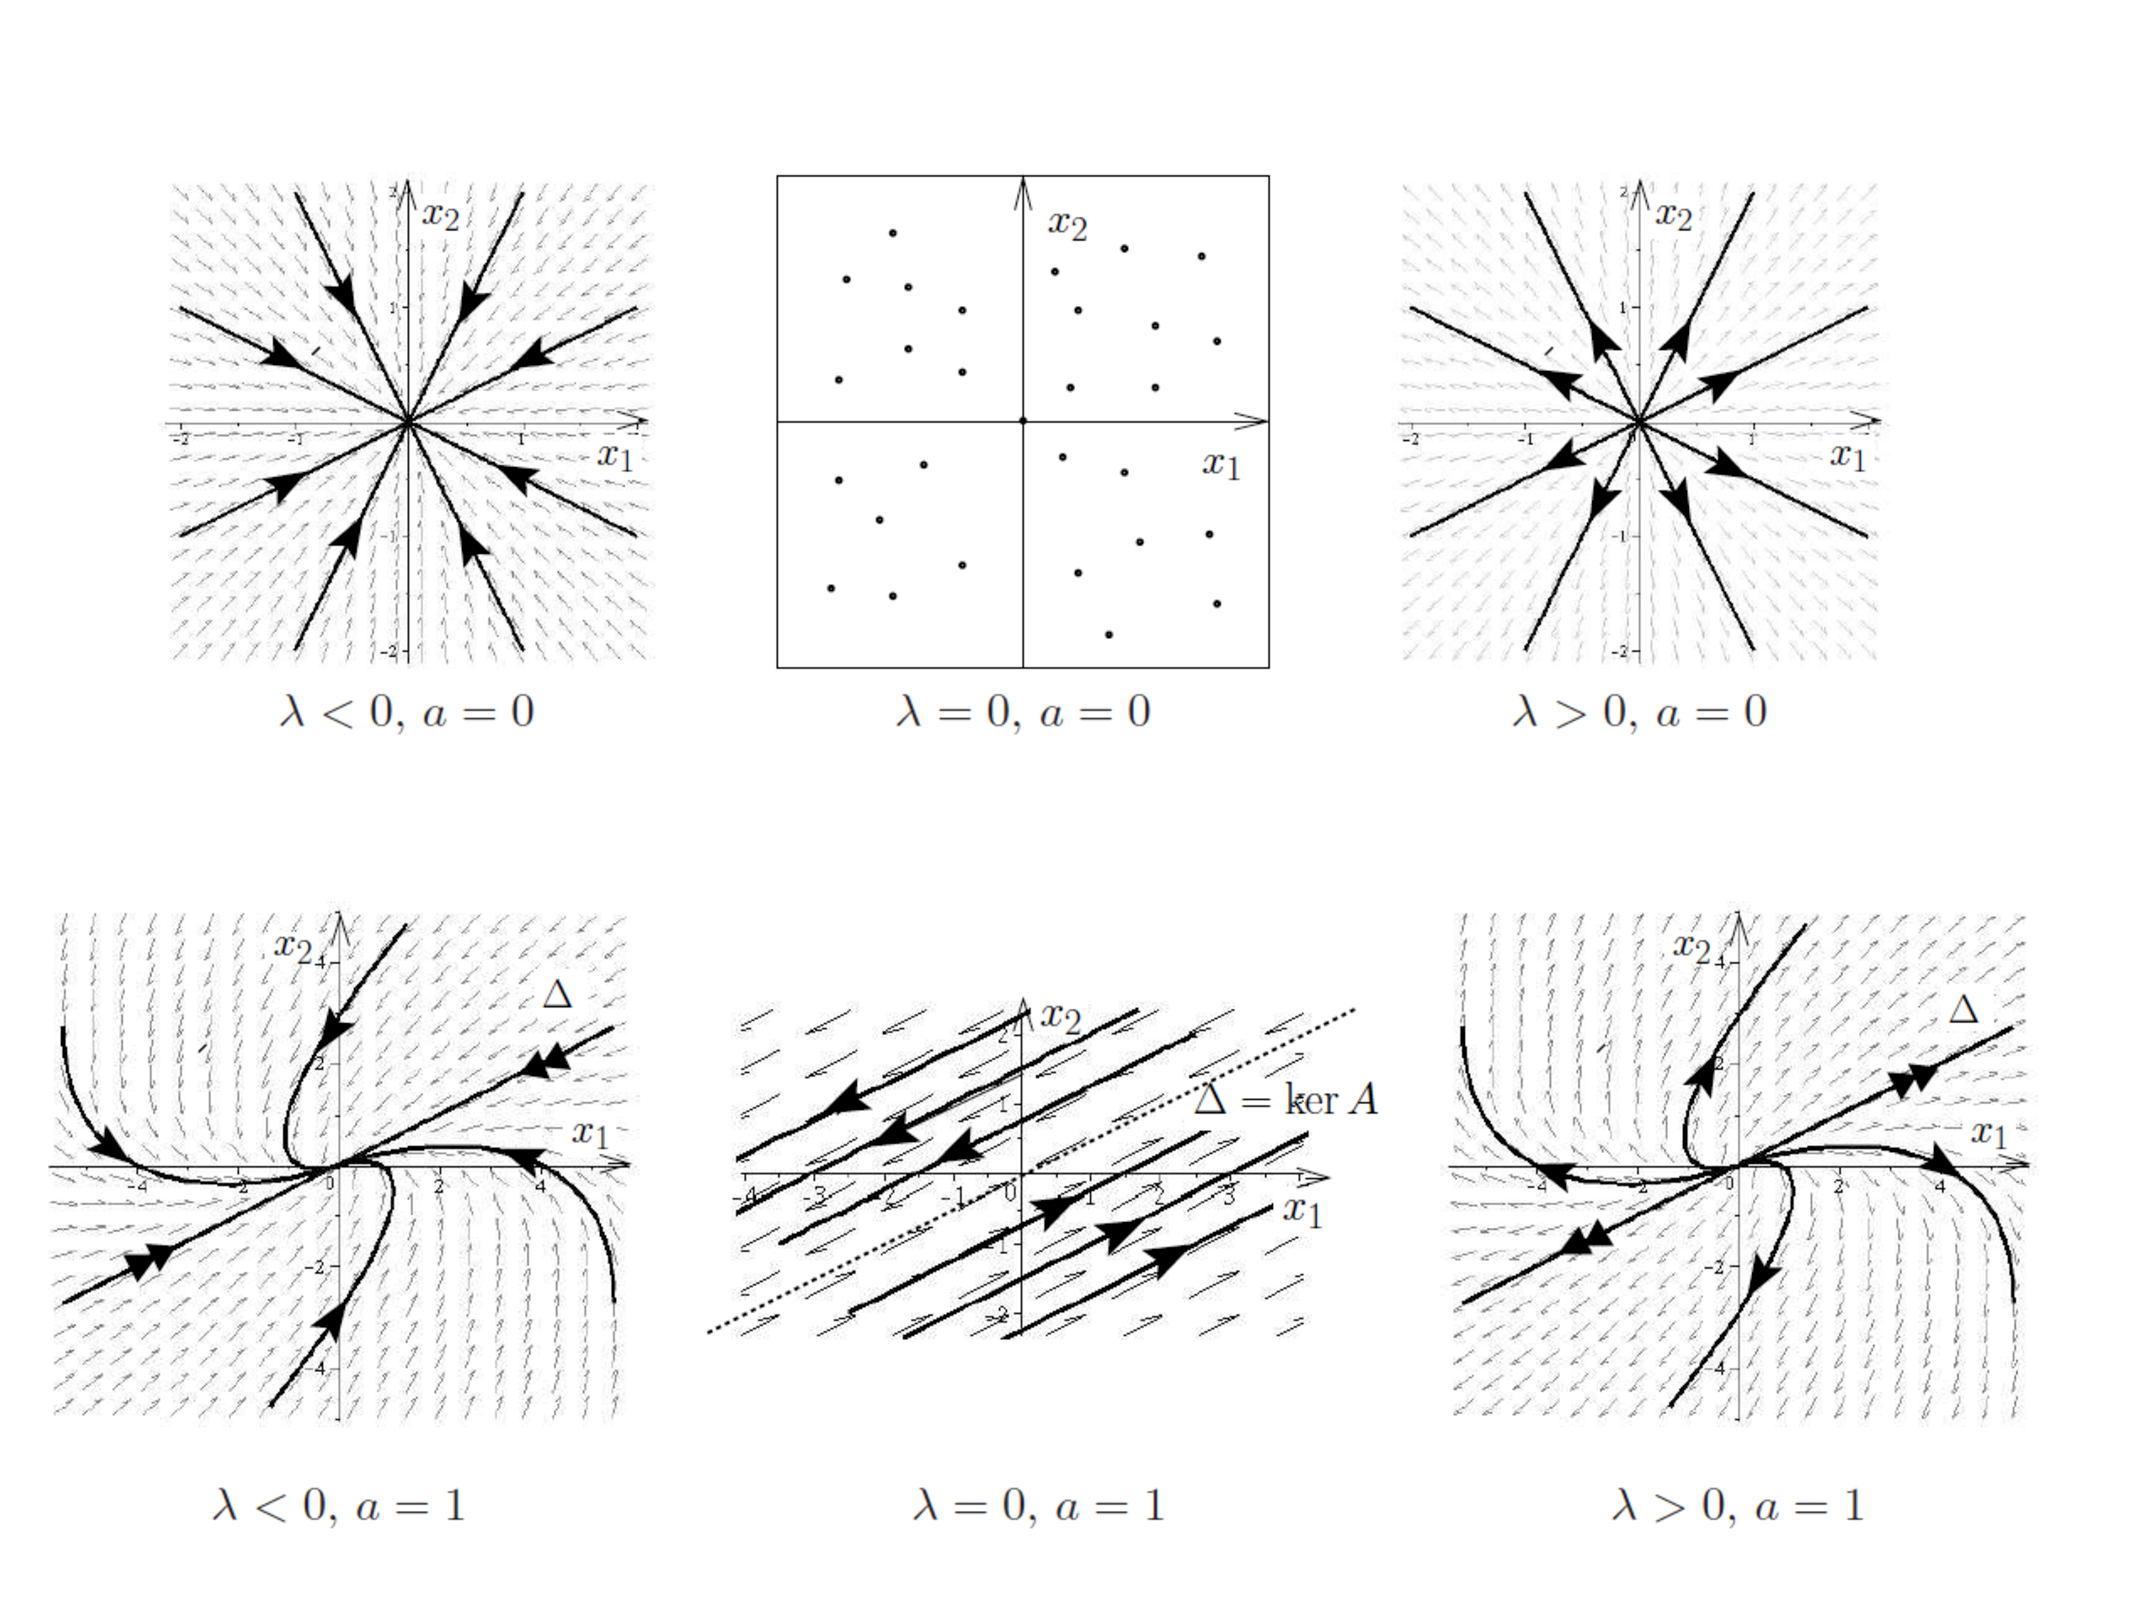
\includegraphics[width=0.7\linewidth]{img/root3.pdf}
  \caption{Various phase portraits for a $2 \times 2$ system in the case of two distinct real roots $\lambda_1, \lambda_2$ (top), in the case of two distinct complex roots $\lambda, \bar{\lambda}$, such that $\Re(\lambda) = \rho$ (middle), in the case of a repeated root $\lambda$ (bottom). When $a = 0$ the dimension of the eigenspace matches the multiplicity ($A$ is actually similar to a diagonal matrix), when $a  = 1$ the dimension of the eigenspace doesn't match the multiplicity ($A$ is similar to an upper triangular matrix).}
  \label{fig:root1}
 \end{figure}

%  \begin{figure}[h!]\label{fig:root3}
%  \centering
%  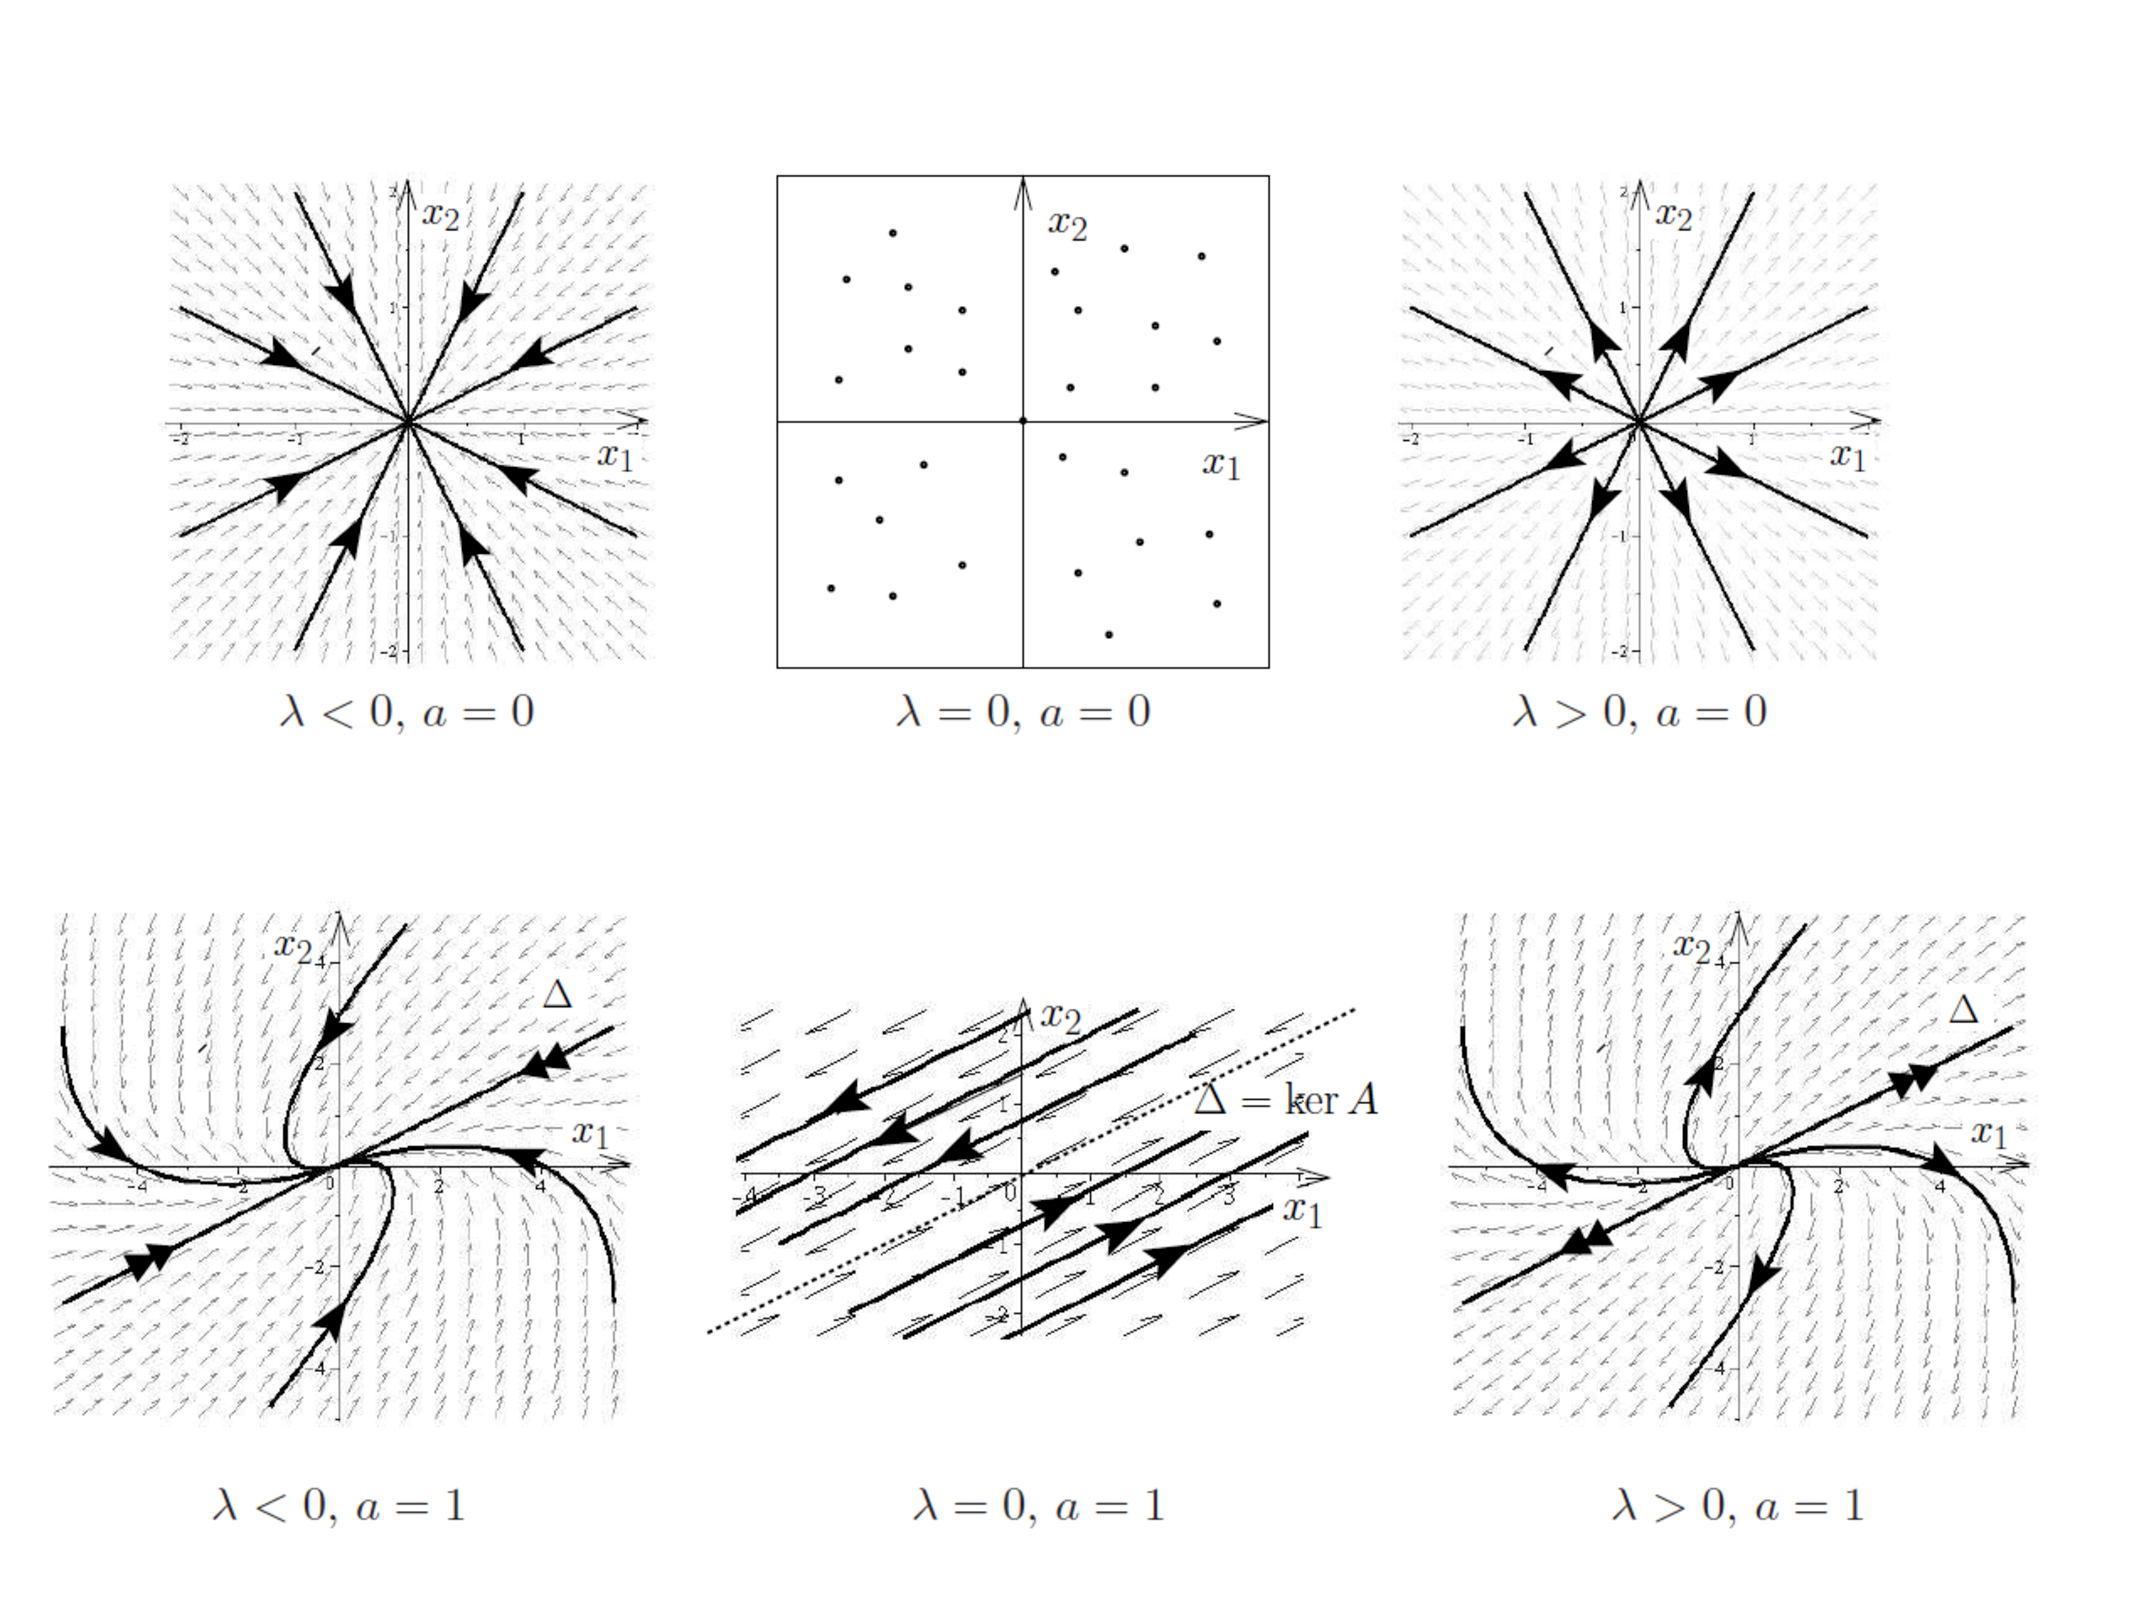
\includegraphics[width=0.8\linewidth]{img/root3.pdf}
%  \caption{Various phase portrait for a $2 \times 2$ system in the case of a repeated root $\lambda$. When $a = 0$ the dimension of the eigenspace matches the multiplicity ($A$ is actually similar to a diagonal matrix), when $a  = 1$ the dimension of the eigenspace doesn't match the multiplicity ($A$ is similar to an upper triangular matrix).}
% \end{figure}
%  \begin{figure}[h!]\label{fig:root2}
%  \centering
%  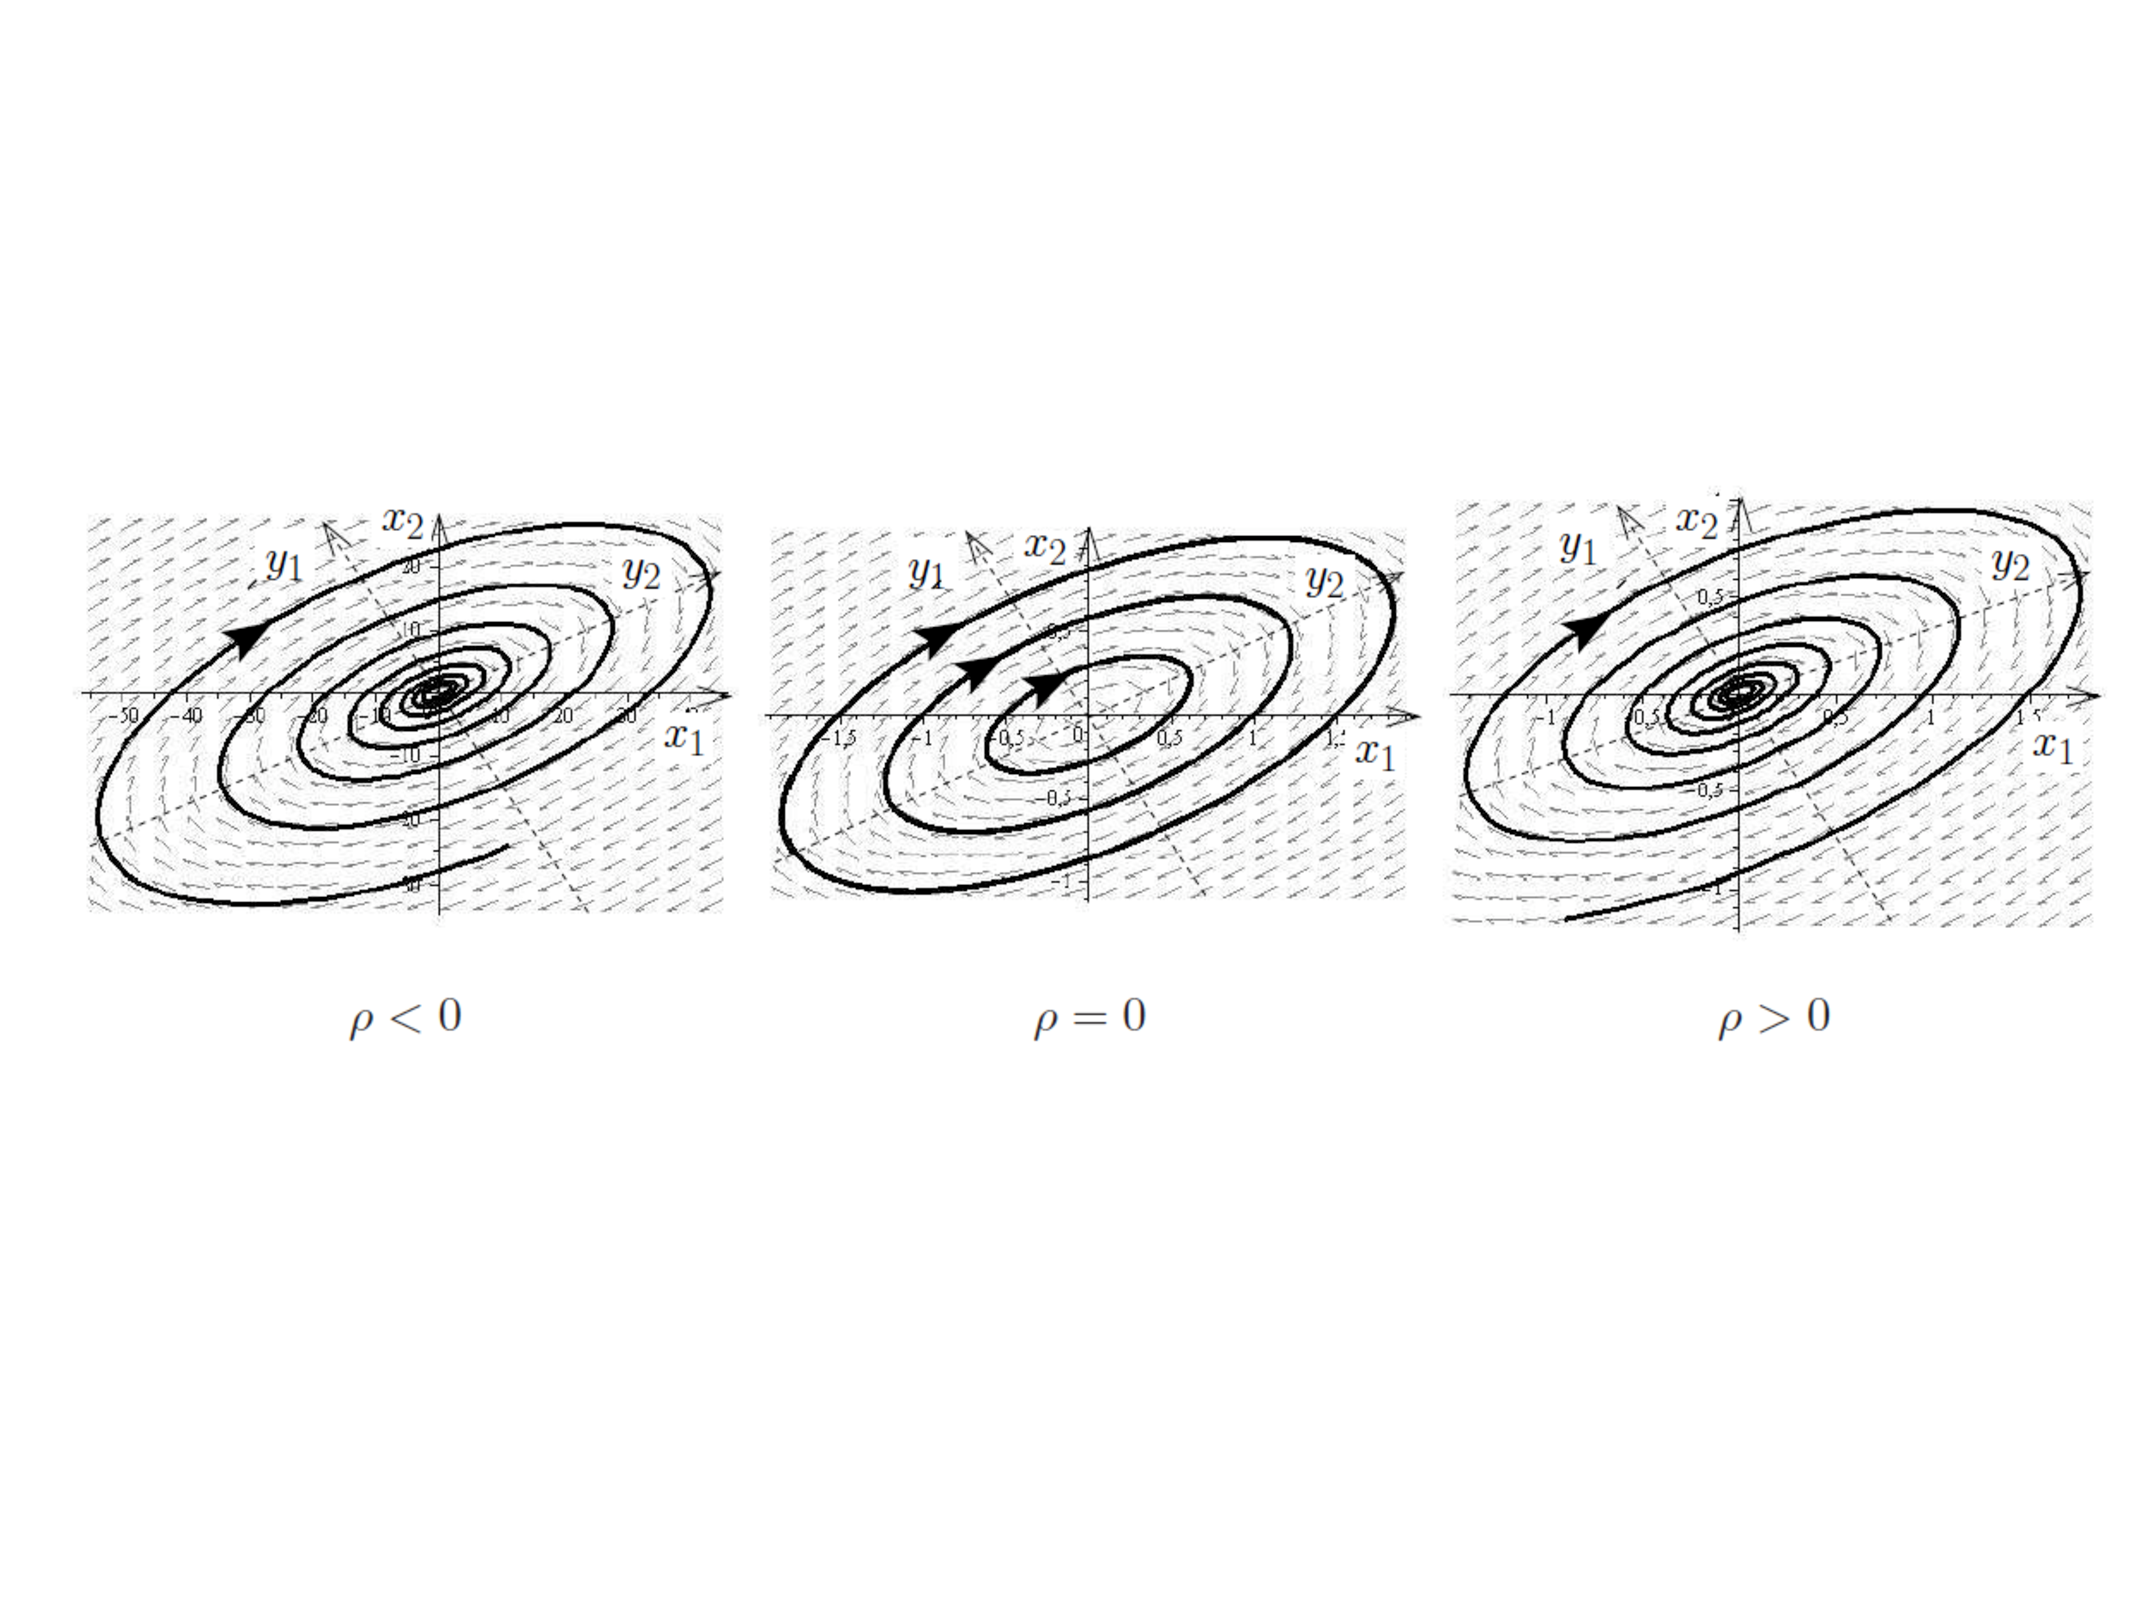
\includegraphics[width=0.8\linewidth]{img/root2.pdf}
%  \caption{Various phase portrait for a $2 \times 2$ system in the case of two distinct complex roots $\lambda, \bar{\lambda}$, such that $\Re(\lambda) = \rho$.}
% \end{figure}

 \begin{Exercise}
Find the equilibrium points, and study their stability and phase portrait for the competitive model \eqref{eq:competitive}.\\
  \dotfill

\dotfill

\dotfill

\dotfill

\dotfill

\dotfill

\dotfill

\dotfill

\dotfill

\dotfill
 \end{Exercise}

\section{Non-dimensionalizing}

We have now investigated multiple population systems, though we have 4 parameters we can change every time we model a new situation. Can we reduce that ? Let's use non-dimensionalizing like in Chapter \ref{chap1}. We define \\
\[ \bar{C} = \gamma C, \quad \bar{F} = \beta F.\]
With this choice we note that $(C,F) = (\frac{1}{\gamma},\frac{1}{\beta})$ is equivalent to $(\bar{C}, \bar{F}) = (1,1)$ !
We need also to non-dimensionalize the variable $t$. We choose for example
\[\tau = \alpha t.\] 
Let's plug now those non-dimensionalized quantities into \eqref{eq:prey-pred}. We obtain 
 \begin{equation}\label{eq:prey-pred_nd}
 \begin{aligned}
&\displaystyle \frac{d \bar{C}}{d \tau} =  \bar{C} \left( 1 - \bar{F}\right)  \\ 
&\displaystyle \frac{d \bar{F}}{d \tau } = -  \frac{\delta}{\alpha}  \bar{F} \left( 1 - \bar{C} \right)  
\end{aligned}
\end{equation}

It turns out that there is only one parameter that is essential for the model, given here by the ratio $\varepsilon = \displaystyle  \frac{\delta}{\alpha} $. It is then recommended to \textbf{non-dimensionalize first} to reduce the number of parameters.\\

Note that choices we made are \textit{homogeneous} in terms of dimensions. First, $ \gamma C$ and $\beta F$ have no dimensions (recall our equilibrium points $(C,F) = (\frac{1}{\gamma},\frac{1}{\beta})$ means that $\frac{1}{\gamma}$,  $\frac{1}{\beta}$ have the same dimension as the number of population $C$, $F$). Second, $\alpha$ and $\delta$ represent growth rates which indicate a rate of change of number of individuals over time ($[\alpha] = [\delta] =  T^{-1}$), which is relevant to use then.

 \begin{Exercise}
Non-dimensionalize \eqref{eq:prey-pred} using this time
\[ \bar{C} = \gamma C, \quad \bar{F} = \beta F, \quad  \tau = \delta t.\]
What do you obtain ?\\
  \dotfill

\dotfill

\dotfill

\dotfill

\dotfill

\dotfill

\dotfill

\dotfill

\dotfill

\dotfill
 \end{Exercise}

\section{Stability via Lyapunov functions}

Stability of equilibrium points via linearized systems is very appealing, but can be cumbersome. We briefly present here another way to establish stability of an equilibrium point (and find its basin of attraction) using Lyapunov functions. Consider the IVP
\[ x' = f(x(t)) ,\quad x(t_0) = \alpha, \quad  a \leq t \leq b,\]
and suppose $x_{eq}$ is an equilibrium point. 
\begin{definition}\label{def:lyap}
Consider a function $L : U \to \mathbb{R}$, where $U$ is a neighborhood of $x_{eq}$. The function $L$ is a Lyapunov function if
\begin{itemize}
\item $L(x_{eq}) = 0$ and $L(x) >0$ for all $x \in U \setminus \lbrace x_{eq}\rbrace $.
\item $\nabla L(x) \cdot f(x) \leq 0$ for all $x \in U$
\end{itemize}
The function $L$ is a strict Lyapunov function if $\nabla L(x) \cdot f(x) < 0$ for all $x \in U \setminus \lbrace x_{eq}\rbrace $.
\end{definition}
\begin{lemma}
Consider a function $L : U \to \mathbb{R}$, where $U$ is a neighborhood of $x_{eq}$. If there exists a Lyapunov function in some vicinity $U$ of $x_{eq}$ then $x_{eq}$ is a stable equilibrium point. If there exists a strict Lyapunov function in the vicinity of $x_{eq}$ then $x_{eq}$ is an asymptotically stable equilibrium point. Additionally $U$ denotes the basin of attraction of the equilibrium point.
\end{lemma}
The basin of attraction represents the region such that, once a trajectory enters this region then it will remain in this region (and in some cases converge towards $x_{eq}$). This approach is then very appealing and much faster than the Jacobian matrix, but the $\$\$\$$ question is: how to find such function $L$ ? It is actually harder than you think. You can win a Fields medal for finding new ones for real-world problems ! Let's discuss one for a simple case.\\

One of the strategies to find such function is based on energy principles. The conditions described in Definition \ref{def:lyap} boil down to $x_{eq}$ being a minimum of the function. If you think about a function of the form $L : x \mapsto (x-x_{eq})^2$ then the first item is automatically satisfied, and $L'(x_{eq}) = 2 (x - x_{eq})$. One may need to check the second condition that will depend on the problem at hand. It is common that energies of systems are quadratic functions (kinetic energy, potentiel energy, etc.), this provides a good candidate to start with.
 \begin{figure}[H]
  \centering
  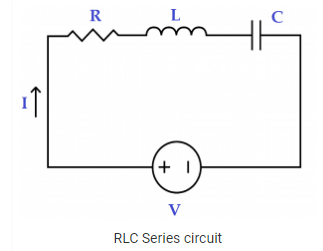
\includegraphics[width=0.4\linewidth]{img/rlc-circuits-in-series.png}
  \caption{Sketch of a RLC circuit.}
  \label{fig:RLC}
 \end{figure}
\begin{Example}
Consider the RLC circuit (see Figure \ref{fig:RLC}) modeled by the telegrapher's equations
\[ 
 \begin{aligned}
&\displaystyle L \frac{d I}{d t} =  V - h(I)  \\ 
&\displaystyle  C\frac{d V}{d t } = - I
\end{aligned}
\]
and we assume $h$ is a function such that $Ih(I) >0$ for all $I \neq 0$, and $h(0) = 0$. Following the procedure we highlighted before one can check that (check it !)
\begin{enumerate}
\item  $(I,V) = (0, h(0) = 0)$ is an equilibrium point.
\item The associated Jacobian matrix is given by $A_{ (0, 0)} = \begin{bmatrix}
 - \frac{h'(0)}{L} & \frac{1}{L} \\ - \frac{1}{C} & 0
\end{bmatrix} $ and admits as eigenvalues $\lambda = - \frac{h'(0)}{2L}\pm  \sqrt{\frac{h'(0)^2 - 4 L}{4 L^2 C}} $.
\item The stability of the equilibrium point depends on $h'(0)$, and we can't conclude as of now.
\end{enumerate}
Let's use a Lyapunov function to determine the stability of the equilibrium. Consider the function
\[E(I,V) = \frac{1}{2} (LI^2 + CV^2)\]
One can check that
\begin{itemize}
\item $E(0,0) = 0$ and $E(I,V) >0 $ for all $(I,V) \neq (0,0)$
\item  $\nabla E (I,V) = \begin{bmatrix}
 L I \\ CV
\end{bmatrix} $ and $F(I,V) = \begin{bmatrix}
-\frac{V - h(I)}{L} \\ - \frac{I}{C}
\end{bmatrix} $. We obtain $ \nabla E (I,V) \cdot F(I,V)  = - VI + I h(I) - IV = I h(I) >0$ by definition.
\end{itemize}
$E$ is then a Lyapunov function (strict), therefore $(0,0)$ is an asymptotically stable. Additionally since the function $E$ satisfies the above conditions for all $(I,V)\in \mathbb{R}^2$, the basin of attraction is the entire plane $\mathbb{R}^2$ !

In this example, no matter what is the initial intensity (I) and voltage (V), after a long time the solution is necessarily $(0,0)$. 
\end{Example}
\begin{Exercise}
Consider the system
 \begin{eqnarray*}
\frac{dx}{dt} &=& x (a- b y -px)  \\
\frac{dy}{dt} &=& y(fx -c - q y)
\end{eqnarray*}
with $a,b,c,f,p,q >0$, and we suppose that $\frac{c}{f} < \frac{a}{p}$.

\begin{enumerate}
\item What kind of model is this system ? Justify.
\item Determine the equilibrium points.
\item We want to discuss the stability of the equilibrium points using a Lyapunov function. Consider the function $L(x,y) = f x^\ast (\frac{x}{x^\ast} - \log (\frac{x}{x^\ast}) -1) +by^\ast (\frac{y}{y^\ast} - \log (\frac{y}{y^\ast}) -1)  $, with $(x^\ast, y^\ast)$ an equilibrium. Determine if $L$ is a Lyapunov function for each equilibrium. If not, what do you conclude ? If yes, what is the attractor region ?
\item Check your answer by studying the eigenvalues of each Jacobian matrix.
\end{enumerate}
\dotfill

\dotfill

\dotfill

\dotfill

\dotfill

\dotfill

\dotfill

\dotfill

\dotfill

\dotfill

\dotfill

\dotfill

\dotfill

\dotfill

\dotfill

\dotfill

\dotfill

\dotfill

\dotfill

\dotfill
\end{Exercise}
\section{Numerical methods}
In practice we will use numerical methods to approximate solutions of dynamical systems. We provide below a very brief summary on how to proceed using Euler's method.\\
Consider the IVP 
 \[ \displaystyle \frac{d y}{d t} = f(y,t), \quad y(0) = \alpha, \quad a \leq t \leq b.\]
 
To idea is to use numerical differentiation: pick an $N$ and discretize the time (and the solution) as follows:
\[ \Delta t = \frac{b-a}{N}, \quad t_j = a + j \Delta t, j = 0,...,N, \quad w_j \approx y(t_j), \quad w_0 = \alpha \]
Then approximate the time derivative as follows:
\[ \displaystyle \frac{d y}{d t}(t_j) \approx \frac{ y(t_{j+1}) - y(t_j)}{\Delta t} \approx \frac{ w_{j+1} - w_j}{\Delta t}.  \] 
The discrete version of the IVP becomes 
\[  w_{j+1} = w_j + \Delta t \, f(w_j, t_j),\quad  j = 0, ...,N, \quad w_0 = \alpha \]

This is Euler's method (the simplest discretization). Runge-Kutta methods are a bit more sophisticated and provide better accuracy, you can also use other multi-step methods such as Adam-Moulton or Adam-Bashforth (review your course material from numerical analysis if needed).

How do we proceed for a system ? Repeat the same approach for each equation in the system Consider for example the system 
 \[ \displaystyle \frac{d y_1}{d t} = f(y_1,y_2,y_3,t), \quad y_1(0) = \alpha, \quad a \leq t \leq b\]
  \[ \displaystyle \frac{d y_2}{d t} = g(y_1,y_2,y_3,t), \quad y_2(0) = \beta, \quad a \leq t \leq b\]
   \[ \displaystyle \frac{d y_3}{d t} = h(y_1,y_2,y_3,t), \quad y_3(0) = \gamma, \quad a \leq t \leq b\]
 which can also be written as
 
 \[ \displaystyle \frac{d Y}{d t}   = \displaystyle \frac{d }{d t}  \begin{bmatrix}
 y_1 \\y_2 \\ y_3
\end{bmatrix}  = F(Y,t)  =  \begin{bmatrix}
 f(y_1,y_2,y_3,t) \\g(y_1,y_2,y_3,t) \\ h(y_1,y_2,y_3,t)
\end{bmatrix}, \quad Y(0) = Y_0 =   \begin{bmatrix}
\alpha \\ \beta  \\ \gamma
\end{bmatrix} , \quad  a \leq t \leq b. \]
Pick an $N$ and discretize the time (and the solution) as follows:
\[ \Delta t = \frac{b-a}{N}, \quad t_j = a + j \Delta t, j = 0,...,N, \quad w_j^k \approx y_k(t_j), k =1,2,3 \] 
\[w_0^1 = \alpha, \quad w_0^2 = \beta, \quad  w_0^3 = \gamma\]
which in vector form corresponds to
\[  W_j  =   \begin{bmatrix}
 w_j^1 \\ w_j^2 \\ w_j^3
\end{bmatrix} \approx Y(t_j) =   \begin{bmatrix}
 y_3(t_j) \\  y_2(t_j) \\  y_3(t_j)
\end{bmatrix}, \quad W_0 =  \begin{bmatrix}
\alpha \\ \beta  \\ \gamma
\end{bmatrix} .\]

The discrete version of the system becomes 
\[  w^1_{j+1} = w^1_j + \Delta t \, f(w^1_j,w^2_j,w^3_j,t_j) ,   \quad  j = 0, ...,N, \quad w_0^1 = \alpha \]
\[  w^2_{j+1} = w^2_j + \Delta t \,  g(w^1_j,w^2_j,w^3_j,t_j),   \quad j = 0, ...,N, \quad w_0^2 = \beta\]
\[  w^3_{j+1} = w^3_j + \Delta t \,  h(w^1_j,w^2_j,w^3_j,t_j),   \quad  j = 0, ...,N, \quad w_0^3 = \gamma \]

What about convergence and stability of the method ? For Euler's method it is well-known that the method converges with a rate of $O(\Delta t)$, however it is quite an unstable method (round-off error play a good role) especially for \textit{stiff systems} (where the step size is constrained to be sufficiently small to maintain stability). It is usually recommended to use higher-order methods such as RK4. \\ 

Recall that the above problem, \textbf{no matter what numerical scheme you choose}, can be rewritten in vector form as 
\[  W_{j+1} = \tilde{F}( W_j ),   \quad  j = 0, ...,N, \quad W_0 =  \begin{bmatrix}
\alpha \\ \beta  \\ \gamma
\end{bmatrix},\]
with $\tilde{F}$ the chosen numerical scheme (for Euler we found $\tilde{F} = F$). The above iterative scheme describes a fixed-point problem, for which we know how to ensure convergence. You may have learned in your numerics class that 
\begin{lemma}\label{lem:fp}
Given a fixed-point problem $x = g(x)$, and associated iterative solver $x_{n+1} = g(x_n)$, $n = 0, \dots, N$, if $|g'(x)| \leq c < 1$ for all $x$ in the domain of interest, then the fixed-point method converges with $O(c^n)$.
\end{lemma}
\begin{proof}
Let's denote $x^f$ the value of the fixed-point: $x^f = g(x^f)$. Then
\[ |x_{n+1} - x^f| = |g(x_{n}) - g(x^f)| \leq \max |g'(x)| |x_n  - x^f|\]
which implies that 
\[ |x_{n+1} - x^f|  \leq c^n |x_0 -x^f|.\]
This is a geometric sequence, and it converges if $c <1$. 
\end{proof}
Ensuring a condition of the form $|g'(x)| \leq c < 1$ implies a condition on the step size $\Delta t$, which guarantees stability of the method in the end. This can be established via the characteristic polynomial associated to $\tilde{F}$.  In what follows we will use this condition to investigate stability of the logistic growth.\\
\begin{remark}
In Python you may use \texttt{scipy.integrate.odeint}, adapted to solve initial value problems for stiff or non-stiff systems of first order ODEs, or \texttt{scipy.integrate.RK45} which approximates an IVP (as a system or not) using Runge-Kutta of order 5(4).
\end{remark}

\begin{remark}
Stability of a numerical scheme and stability of an equilibrium point are not exactly the same.  Stability of an equilibrium point can be found by studying the sign of the eigenvalues of the \textbf{Jacobian matrix}, whereas stability of a numerical method can be found by studying the \textbf{sign of the roots of the characteristic polynomial from the numerical scheme}. The roots and eigenvalues in question are not the same ! 
\end{remark}
\section{Logistic map: towards chaos}

In the previous section we discussed that the numerical stability of the method is in fact conditioned by the size of the step size $\Delta t$, related to some fixed-point constraint to ensure convergence. In this section we provide an example for the logistic growth.\\

Consider the non-dimensionalized logistic growth model:
\[ \displaystyle \frac{d y}{d t} = y (1- y)\]
Using the same notations as before, applying Euler's method provides the following discrete scheme
\[ \displaystyle w_{n+1}=w_n + \Delta t ( w_n (1- w_n) ) = (1 + \Delta t) w_n (1 - \frac{\Delta t }{1 + \Delta t} w_n)\]
We now define
\[x_n =  \frac{\Delta t }{1 + \Delta t} w_n, \quad \beta = (1 + \Delta t)  >1\]
 and rewrite the above numercial scheme as 
 \[x_{n+1} = f(x_n )= \beta x_n (1- x_n).\]
 The above function $f$ is called the \textit{logistic map}. This is a fixed-point problem and we know that it admits the fixed points
 \[x^f = 0, \quad x^f = \frac{\beta -1 }{\beta} >0\]
 From Lemma \ref{lem:fp} we need to check that $|f'(x)| < 1$ to guarantee convergence. We obtain:
 \[f'(x) = \beta (1 - 2 x) \quad \Longrightarrow |f'(x)| < 1 \, \Longleftrightarrow \, \Delta t < \frac{1}{|1- 2x|} -1 \]
 which provides constrains on the step size.
 Note that in particular that at the equilibrium point we obtain
 \[\Delta t < \frac{1}{|1- 2 \times 0|} -1 = 0 \mbox{ contradiction} \]
 so we can't guarantee convergence towards $0$. Then we also have
  \[\Delta t < \frac{1}{|1- 2 \times \frac{\beta -1}{\beta}|} -1 <1 \quad \Longleftrightarrow 1 < \beta < 3 \mbox{ therefore } 0 <  \Delta t < 2.\]
  We have then obtained a condition on the time step to guarantee convergence.  Exercise \ref{ex:lm} allows to represent the iterations of the fixed point for various $\beta$. One of them corresponds to a peculiar case: $\beta = 4$. This case is out the stability range we obtained earlier so we already know it won't be convergent. However this case is very peculiar: it is known as \textit{chaotic}. The solution is really unstable and is completely unpredictable. This is a really interesting case of chaotic regime ! Other common cases include the Lorentz attractor:
  \[\begin{aligned}
  x' & = \sigma (x-y)\\
  y' & = x(\rho -z) - y \\
  z'  &= xy - \beta z
  \end{aligned}
  \]
  with $\sigma, \rho, \beta >0$. 
  We highly recommend to take a look at \url{https://matplotlib.org/3.2.1/gallery/mplot3d/lorenz_attractor.html} for an example in Python.
\begin{Exercise} \label{ex:lm}
Figure \ref{fig:log} represents the functions $y = x$ and $y = \beta x(1-x)$ for various $\beta$. Sketch the iterations when solving the fixed-point $x = \beta x(1-x) $ starting at $x_0 = 0.2$. Comment your observations.
 \begin{figure}[h]
  \centering
  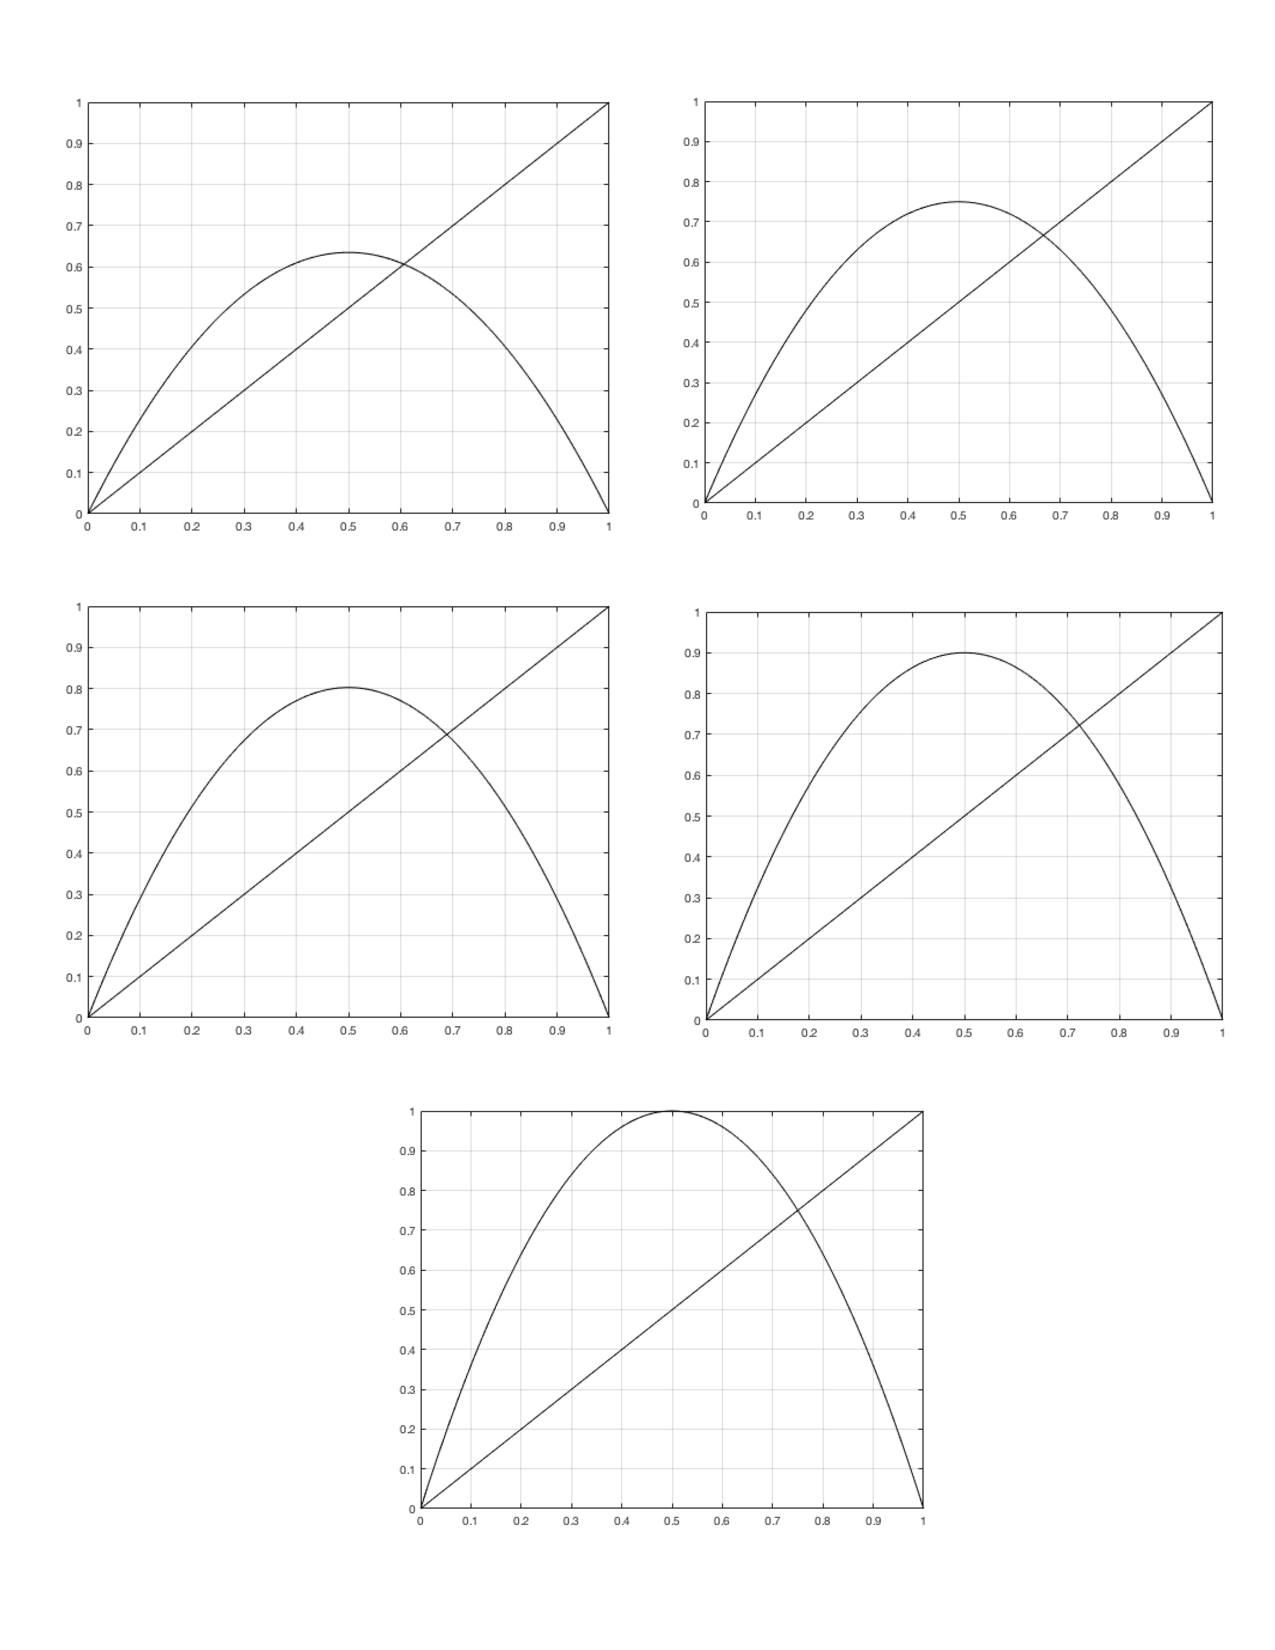
\includegraphics[width=0.9\linewidth]{img/logisticmap_empty.pdf}\\
  \caption{Several logistic maps with various $\beta$.}
  \label{fig:log}
 \end{figure}
 \end{Exercise}
 
 \begin{Exercise} 
Consider the Lorenz attractor
  \[\begin{aligned}
  x' & = \sigma (x-y)\\
  y' & = x(\rho -z) - y \\
  z' & = xy - \beta z
  \end{aligned}
  \]
  with $\sigma, \rho, \beta >0$.  Identify its equilibrium points and study their stability. Try numerically the parameters $\sigma  = 10$, $\rho = 28$, and $\beta = \frac{8}{3}$. What do you observe ? You may use classic codes online such as \url{https://alpha.iodide.io/notebooks/2275/?viewMode=report}.\\
  \dotfill

\dotfill

\dotfill

\dotfill

\dotfill

\dotfill

\dotfill

\dotfill

\dotfill

\dotfill
 \end{Exercise}
 
\section{Conclusion}
In this Chapter  we saw that differential equations is a great tool to model evolution of species, and there is a large applications in economics, population dynamics, physics and others. It is important to look for equilibrium points, study their stability to predict long term behaviors and trajectories based on initial conditions. Keep in mind that numerical methods such as Euler, RK or multi-step methods are efficient techniques to find an approximation to the complex system you may want to solve, however be careful with their numerical stability (pick an appropriate step size). While the model can work in theory, sometimes you encounter chaotic systems and there is nothing you can do about it...\\
We finish with some remarks:
\begin{itemize}
\item We chose ODEs here to track evoluation over time. For spatio-temporal variations we may use Partial Differential Equations. This will require new discretization schemes in space, but we can built on what we have.
\item It is important to investigate perturbations of the model (stability of the numerical scheme, robustness of the method), and compare to realistic data.
\item It is essential as well to question the complexity of our model: how can we track of other variations ? How to develop large-scale tracking ? What resources do we have to compute our model ?
\item Realistic data contains errors (measurements are not perfect), there is a need to add uncertainty into our model. The key is then to introduce some randomness, and noise. The following chapter provides the first step to do so.
\end{itemize}
 
 
 
 
 